\documentclass[11pt]{article}
\usepackage[utf8]{inputenc}
\usepackage{amsmath}
\usepackage{amssymb}
\usepackage{titlesec}
\usepackage{titling}
\usepackage{geometry}
\usepackage{graphicx}
\usepackage{hyperref}
\usepackage{float}
\usepackage{fancyhdr}
\usepackage{wallpaper}
\usepackage{afterpage} 
\usepackage{pagecolor} 
\usepackage{multirow}
\usepackage{wrapfig}
\usepackage{lipsum} 
\usepackage{url}
\usepackage[toc,page]{appendix}
\usepackage{algorithm}
\usepackage{algpseudocode}
\usepackage{pgfgantt}
\usepackage{tabularx}
\usepackage{graphicx}
\usepackage[numbers]{natbib}
\usepackage{url} 
\usepackage{subfig}
 
% Define colors
\usepackage{xcolor}
\definecolor{myblue}{RGB}{33, 66, 99}
\definecolor{mygray}{RGB}{169, 169, 169}
\definecolor{darkbluegrey}{RGB}{44, 62, 80} 

% Page styling
\pagestyle{fancy}
\fancyhf{}
\renewcommand{\headrulewidth}{0pt}
\renewcommand{\footrulewidth}{0pt}
\fancyfoot[C]{\thepage}
\renewcommand{\familydefault}{\sfdefault}

% Define a command for section headers
\titleformat{\section}
  {\color{myblue}\normalfont\Large\bfseries}
  {\color{myblue}\thesection}{1em}{}

% Define a command for subsection headers
\titleformat{\subsection}
  {\color{myblue}\normalfont\large\bfseries}
  {\color{myblue}\thesubsection}{1em}{}

% Adjust page margins
\geometry{a4paper, margin=1in}

% make references clickable
\hypersetup{
    colorlinks=true,
    linkcolor=blue,
    filecolor=magenta,      
    urlcolor=cyan,
}

\begin{document}

% Change the background color of the first page
\pagecolor{darkbluegrey}
\afterpage{\nopagecolor}

% Add a background image
\ThisCenterWallPaper{0.75}{./image/ferrofluide.png}

\begin{titlepage}
  \vspace*{\stretch{1}}
  \begin{center}
    \textcolor{white}{\textbf{\Huge Final Report}}\\
    \vspace{1cm}
    \textcolor{white}{\Large Spiking Neural Networks\\Sound Detection and Classification}
    \vspace{3cm}
  \end{center}
  \vspace*{\stretch{2}}
  \begin{center}
    \textcolor{white}{
      \textbf{COURREGE Téo}\\
      \textbf{GANDEEL Lo'aï}\\
      \vspace{1cm}
      \Large Date: \today}
  \end{center}
  \vspace*{\stretch{1}}
\end{titlepage}

\newpage

\tableofcontents

\pagebreak

\listoffigures

\pagebreak

\section{Introduction}

\begin{figure}[ht]
  \begin{minipage}[b]{0.45\textwidth}
    In the last report, we explored the foundational aspects of Spiking Neural Networks (SNNs) and their potential applications, focusing on audio classification tasks. We delved into the theoretical underpinnings of SNNs, studying various neuron models and encoding methods such as rate, latency, and frequency coding. Additionally, we addressed challenges related to data preprocessing, verification, and the reconstruction of audio signals using Mel-frequency cepstral coefficients (MFCCs).
  \end{minipage}
  \hfill
  \begin{minipage}[b]{0.5\textwidth}
    \centering
    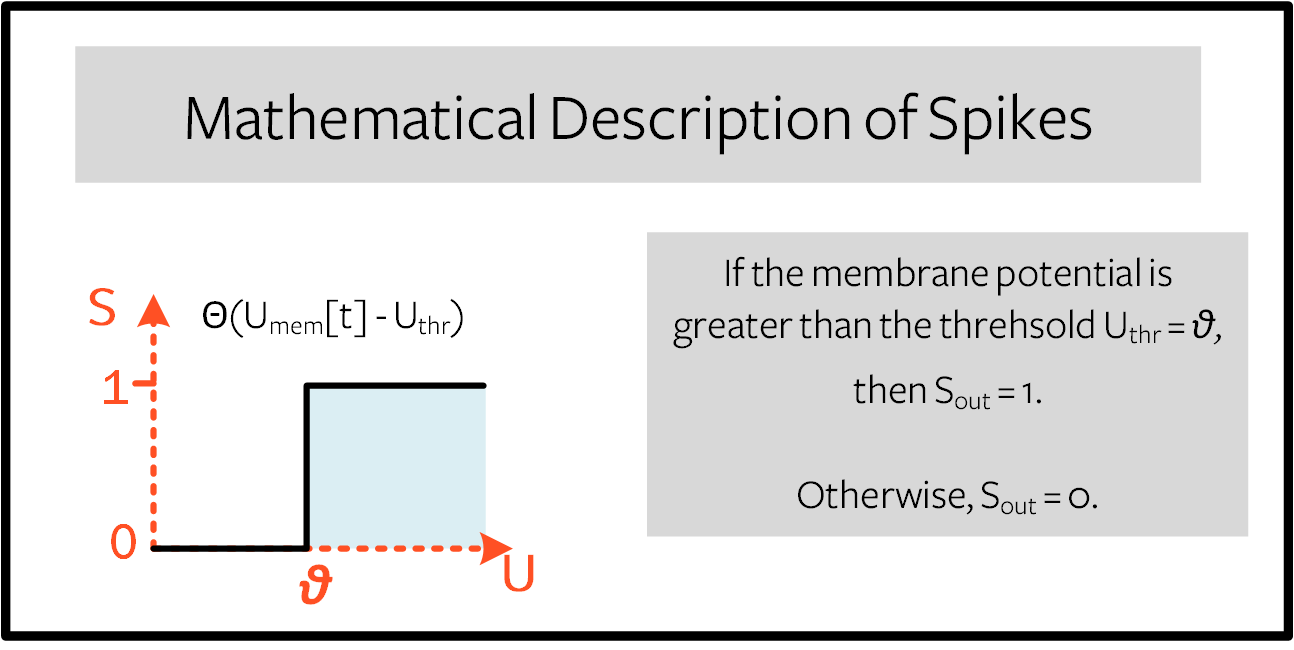
\includegraphics[width=\textwidth]{./image/spike_description.png}
    \caption{Mathematical description of a Spike\cite{eshraghian2021training}}
    \label{fig:spike_description}
  \end{minipage}
\end{figure}

Building upon this foundation, the current report will delve deeper into the intricacies of SNNs, specifically addressing the non-differentiability issue inherent in these networks. Non-differentiability poses a challenge in applying traditional gradient-based optimization techniques commonly used in training Artificial Neural Networks (ANNs). We will explore strategies to tackle this issue and optimize SNNs effectively.

Furthermore, we will introduce the concept of Convolutional Spiking Neural Networks (CSNNs), extending the discussion beyond simple SNN architectures. CSNNs leverage the spatial hierarchies present in convolutional neural networks (CNNs) and integrate them with the temporal dynamics of SNNs. This fusion holds promise for tasks like image recognition, where both spatial and temporal features play crucial roles.

In the practical implementation section, we will present a small program showcasing our results. This program will include the application of CSNNs in a specific task, demonstrating the capabilities and potential advantages of this hybrid architecture.

Throughout this report, our aim is to provide a comprehensive understanding of the advancements and challenges in the realm of Spiking Neural Networks, offering insights into their unique characteristics and applications.

\pagebreak

\section{Reminder on Spikes and Spiking Neural Networks}

Through this section, we aim to provide a comprehensive and visual view of the concepts and mechanisms behind Spiking Neural Networks (SNNs). We will start by revisiting the fundamental aspects of spikes and their encoding, followed by an overview of neuron models (more specifically the Leaky Integrate-and-Fire (LIF) neuron model). We will then delve into the architecture of SNNs and their convolutional variant, Convolutional Spiking Neural Networks (CSNNs).

\subsection{Spikes encoding}

The idea behind spikes is simple: we need to encode some data (let's say an image) into some other kind of data that has a temporal dependency. To do so, we will need to define time steps, a number of steps, and a threshold.
In a rate encoding scheme, we take the values of the pixels of the image and make them pass through a function that will output or not a spike (for example, a Bernoulli function).


\begin{figure}[ht]
  \centering
  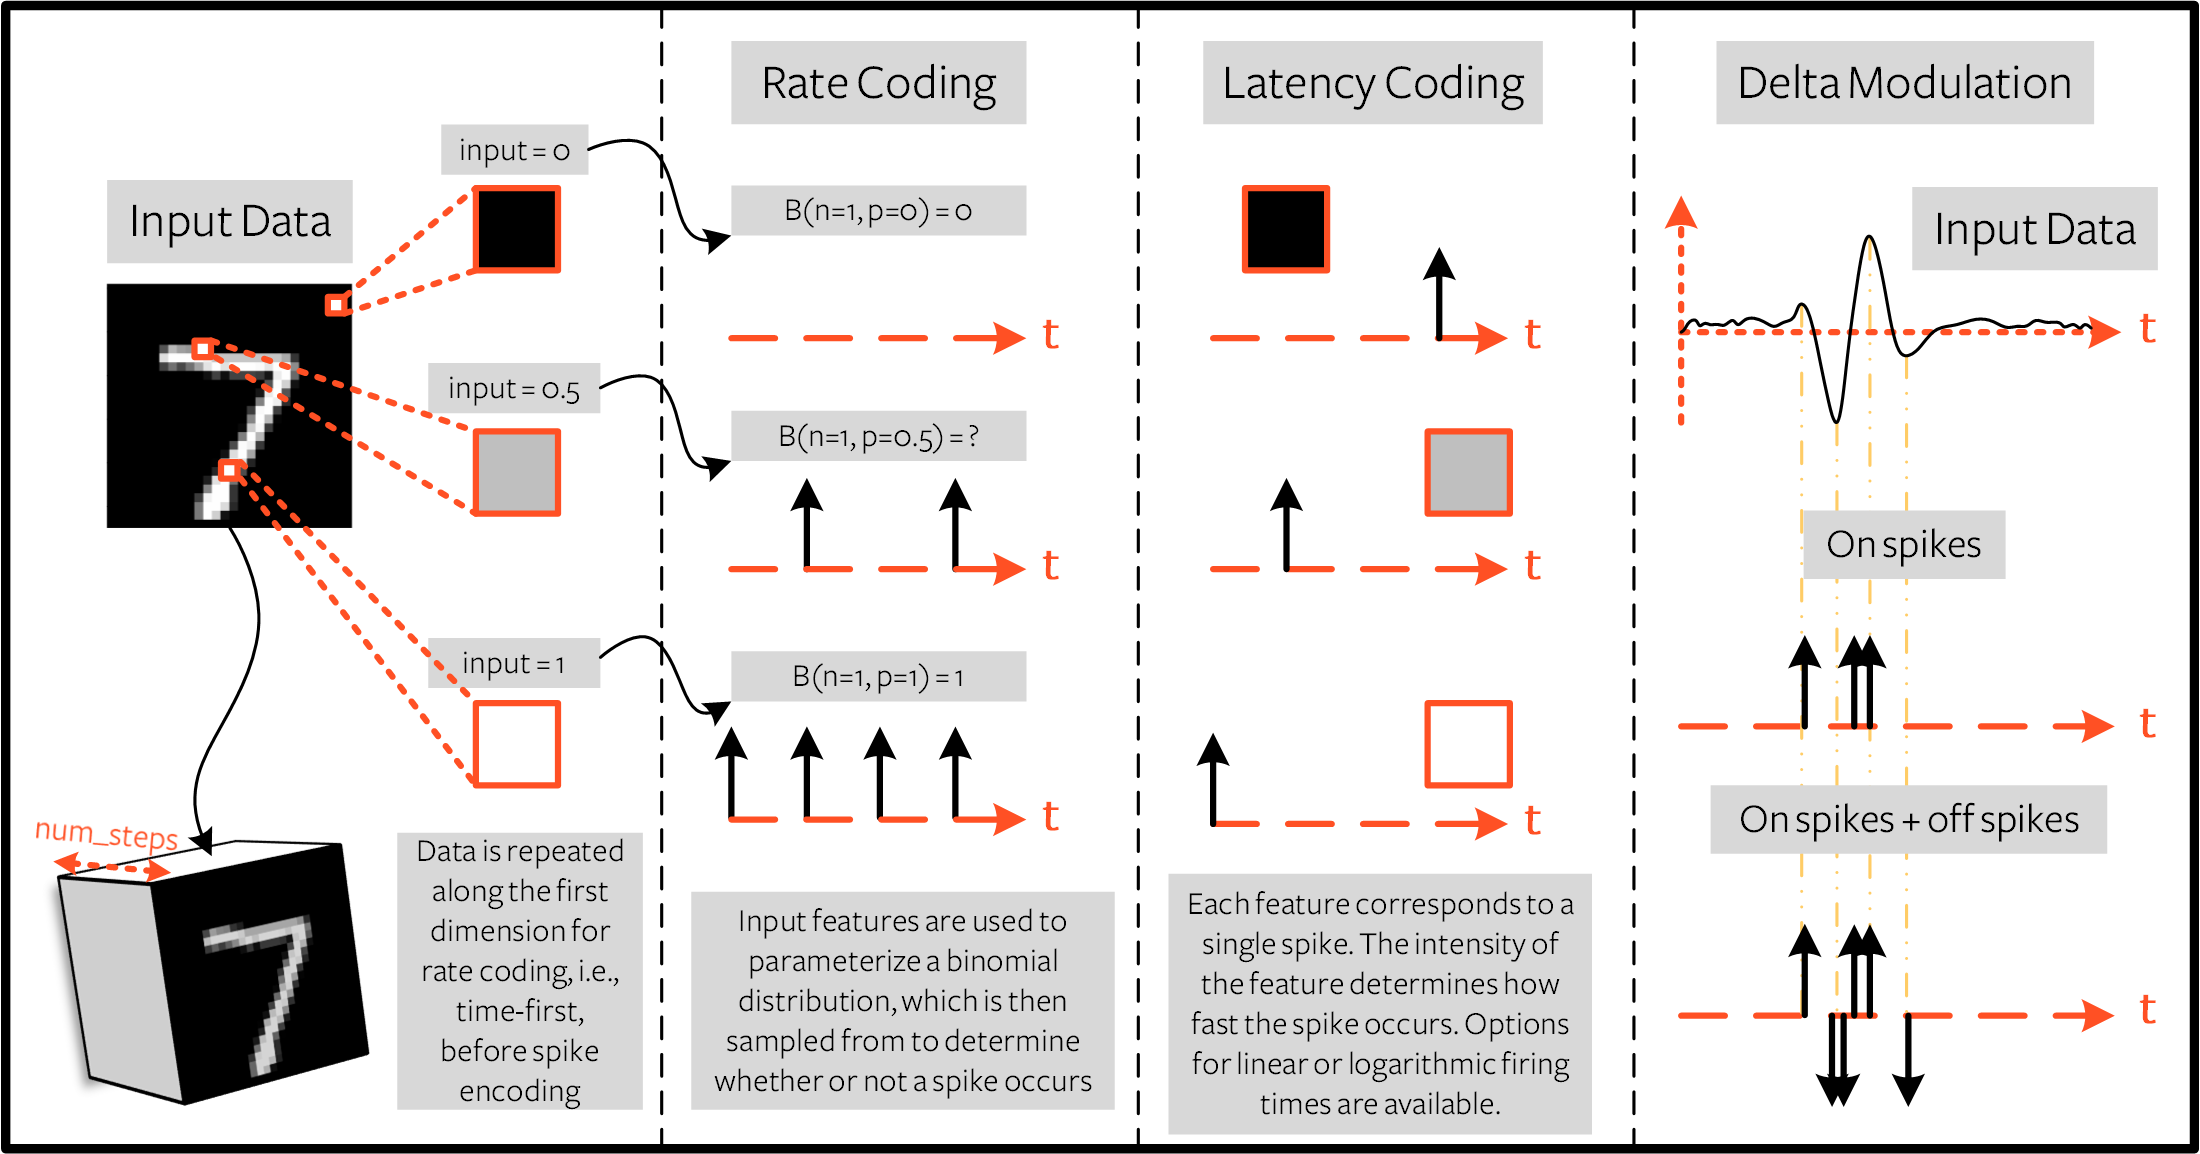
\includegraphics[width=\textwidth]{./image/spikeconv.png}
  \caption{Spike encodings of an image \cite{eshraghian2021training}}
  Source : \url{https://snntorch.readthedocs.io/en/latest/tutorials/tutorial_1.html}
  \label{fig:spikeconversion}
\end{figure}

\subsubsection{Rate encoding}

\subsubsection*{Example}

The rate encoding will for each neuron at each time step, have a probability to fire a spike ($1$) or not ($0$) given by a Bernoulli distribution, where p is proportional to the intensity of the pixel associated with the neuron,.


$$P(X = x) = p^x (1 - p)^{1-x} \quad \text{for } x \in \{0, 1\}$$



Let's say we have a white pixel (value close to $1$) and a black pixel (value close to $0$). The white pixel always emits a spike while the black pixel never fires. In the case of a grey pixel, let's say with intensity of 0.5, when the number of time steps increases, we see that the neuron fires one out of two time steps on average.

This way, we end up with an approximation of the image in the form of spikes (binary values !). In order for it to be efficient, we will need encode the image multiple times. So, we will encode the image using the same method but with different time steps:

\begin{figure}[H]
  \centering
  \begin{minipage}{0.3\textwidth}
    \centering
    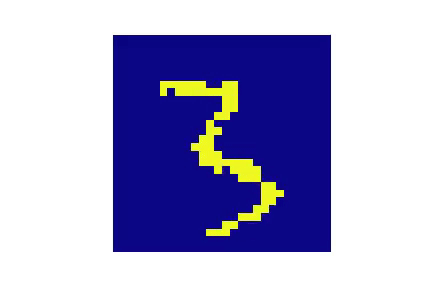
\includegraphics[width=1\textwidth]{image/rate_gif-0.png}
    \caption{MNIST\cite{eshraghian2021training} $t=0$}
    \label{fig:rate_t_0}
  \end{minipage}
  \hfill
  $\xrightarrow{\hspace*{0.3cm}}$
  \hfill
  \begin{minipage}{0.3\textwidth}
    \centering
    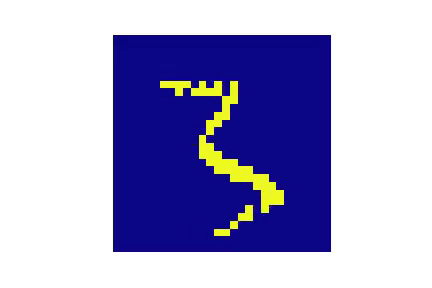
\includegraphics[width=1\textwidth]{image/rate_gif-15.png}
    \caption{MNIST\cite{eshraghian2021training} $t=15$}
    \label{fig:rate_t_15}
  \end{minipage}
  \hfill
  $\xrightarrow{\hspace*{0.3cm}}$
  \hfill
  \begin{minipage}{0.3\textwidth}
    \centering
    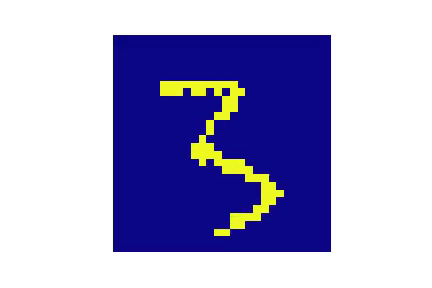
\includegraphics[width=1\textwidth]{image/rate_gif-32.png}
    \caption{MNIST\cite{eshraghian2021training} $t=32$}
    \label{fig:rate_t_32}
  \end{minipage}
\end{figure}

We would define a number of time steps $n_{\text{steps}}$ and encode the image $n_{\text{steps}}$ times. The more time steps we have, the more precise the encoding will be :

\begin{figure}[H]
  \begin{center}
    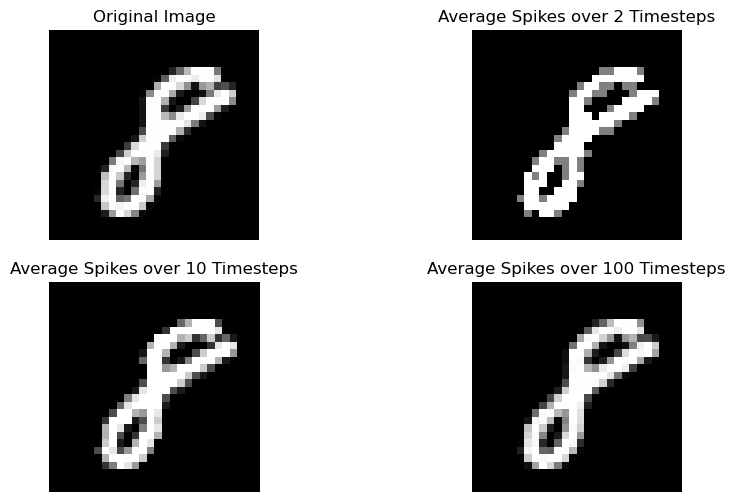
\includegraphics[width=0.8\textwidth]{./image/avg_mnist_spike.png}
    \caption{Average of the encoding of the MNIST dataset}
    \label{fig:avg_mnist_spike}
  \end{center}
\end{figure}

\subsubsection{Latency encoding}

Here the intensity of the pixel is related to the spike timing with a logarithmic dependency, a brighter pixel will spike earlier than a darker one.

This encoding induces more sparsity, but is more prone to have perturbation related errors, as each spike carries way more information than with the rate encoding.



\subsubsection{Decoding}

For the output we need to convert spikes into something the network can interpret. Outputs neurons take input spikes and depending on the encoding chosen will have different behavior.

\begin{itemize}
  \item Rate coding: the predicted class corresponds to the output neuron with the most spikes fired.
  \item Latency coding: the predicted class correspond to the output neuron that fire the first.
\end{itemize}



\subsection{Spiking neuron models}

Another important aspect of Spiking neural network would concern the transmission of spikes and their associated information to the next layer.

We can basically distinguish three phases in a spiking neural network, 2 of them will be explicit later on in the report :
\begin{itemize}
  \item Encoding the data into spikes :

        Converting the input data into spikes (binary values that have approximatly the same "meaning" as the input data, but in a different form), using a specific encoding method (rate, latency, delta modulation, etc.)

  \item Transmitting the spikes (and their associated information) to the next layer :

        Allowing for an information to go further in the network iff the neuron fires a spike (ie. if the feature is important enough to be transmitted to the next layer), kind of imitating the role of an activation function in an ANN.

  \item Decoding the spikes into a meaningful output :

        For a classification task, it would involve firing or not a spike in the output layer (multiple neurons of this final layer can fire at the same time). The neuron that would fire the most over time would be the one associated to the predicted class.
\end{itemize}

To do so, we would need a type of neuron that "fires" spikes when it receives enough input (whatever the inputs are). One might find different kinds of neurons, each with its own characteristics and properties.

\begin{figure}[H]
  \begin{center}
    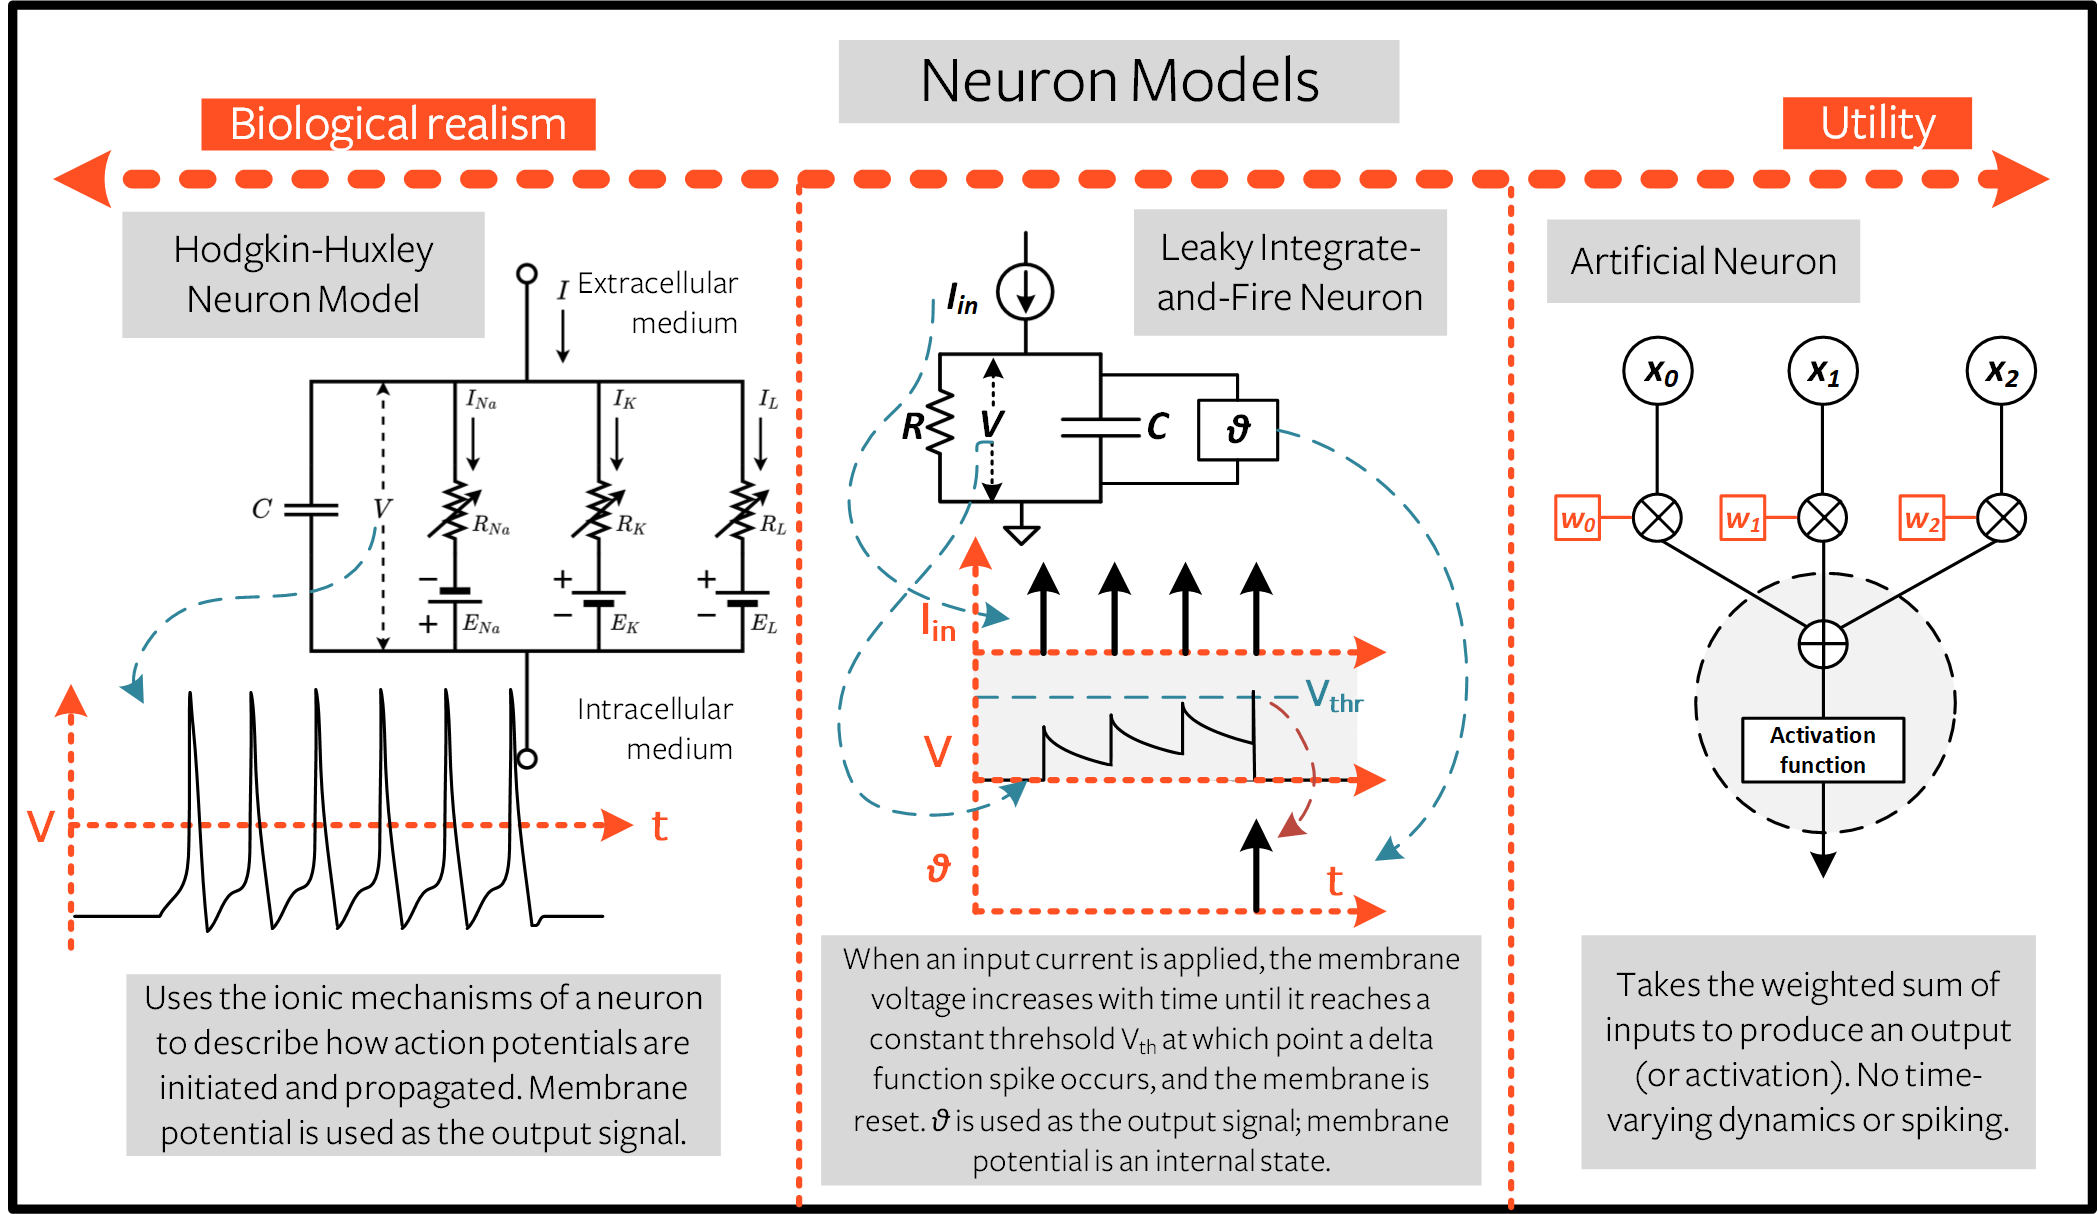
\includegraphics[width=\textwidth]{./image/2_1_neuronmodels.png}
    \caption{Neuron models with schemes}
    \label{fig:neuronmodels_schemes}
  \end{center}
\end{figure}

\subsubsection{Comparison of the different neuron models}

\begin{figure}[H]
  \begin{center}
    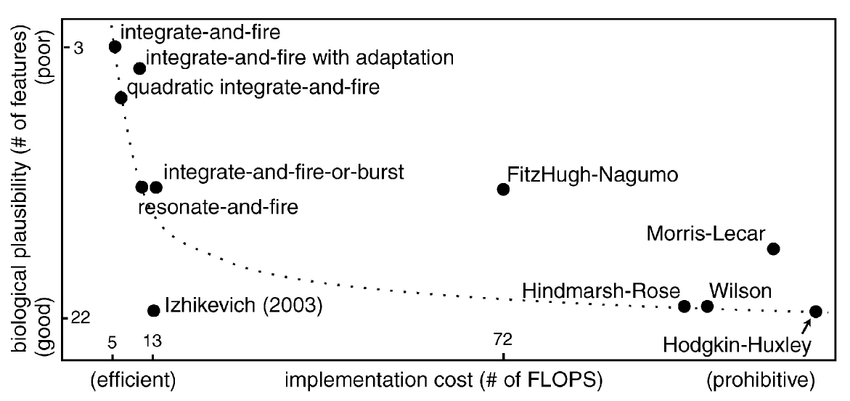
\includegraphics[width=0.8\textwidth]{./image/comparison_neuron.png}
    \caption{Comparison of the different neuron models}
    \label{fig:comparison_neuron}
    Source: \url{https://www.researchgate.net/figure/Trade-off-between-biological-plausibility-with-respect-to-a-number-of-features-known-to_fig3_320409442}
  \end{center}
\end{figure}

\subsubsection{The choice of the Leaky Integrate-and-Fire Neuron Model}

Initially, the LiF model was made as a simple model to mimic the behavior of a neuron.
\begin{quote}
  "In order to arrive at an equation that links the momentary voltage $u_i(t) - u_{rest}$ to the input current $I(t)$, we use elementary laws from the theory of electricity. A neuron is surrounded by a cell membrane, which is a rather good insulator. If a short current pulse $I(t)$ is injected into the neuron, the additional electrical charge $q= \int I(t')dt'$ has to go somewhere: it will charge the cell membrane. The cell membrane therefore acts like a capacitor of capacity $C$. Because the insulator is not perfect, the charge will, over time, slowly leak through the cell membrane. The cell membrane can therefore be characterized by a finite leak resistance $R$.

  The basic electrical circuit representing a leaky integrate-and-fire model consists of a capacitor $C$ in parallel with a resistor $R$ driven by a current $I(t)$ (cf the LiF \hyperref[fig:comparison_neuron]{"Neuron models with schemes"})"\cite{gerstner2014neuronal}
\end{quote}

\begin{figure}[H]
  \begin{minipage}{0.5\textwidth}
    \centering
    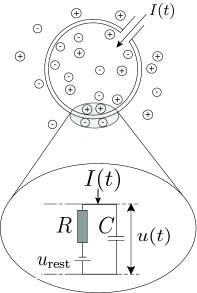
\includegraphics[width=0.6\linewidth]{image/x12.png}
    \caption{A neuron, which is enclosed by the cell membrane (big circle), receives a (positive) input current $I(t)$
      which increases the electrical charge inside the cell. The cell membrane acts like a capacitor in parallel with a resistor which is in line with a battery of potential $u_{rest}$\cite{gerstner2014neuronal}}
    \label{fig:neuron_real_circuit}
  \end{minipage}
  \hspace{0.5cm}
  \begin{minipage}{0.5\textwidth}
    \centering
    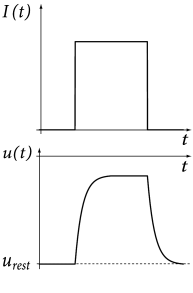
\includegraphics[width=0.6\linewidth]{image/x13.png}
    \caption{The cell membrane reacts to a step current (top) with a smooth voltage trace (bottom)\cite{gerstner2014neuronal}}
    \label{fig:neuron_real_circuit_trace}
  \end{minipage}
\end{figure}

From the Ohm's law and the capacitance equation, we can derive the following equation :

\begin{equation}
  \implies RC \frac{du(t)}{dt} = -\left[u(t) - u_{rest} \right] + RI(t)
\end{equation}

Say the neuron starts at some value $u_{0}$ with no further input, i.e., $I(t)=0$. The solution of the linear differential equation is:

$$u(t) = u_0e^{-\frac{t}{\tau}}$$

Where $\tau = RC$ is the time constant of the neuron. This equation shows that the membrane potential decays exponentially to zero with a time constant $\tau$.

\subsubsection{Leaky Integrate-and-Fire Neuron Model}

With the Leaky Integrate-and-Fire (LIF) model been the most used in practice. It can be seen as follows :

\begin{itemize}
  \item We define a membrane potential $U_m$ that will be updated at each time step
        \begin{equation}
          U_m[t+1] = \underbrace{\beta U_m[t]}_\text{decay} + \underbrace{WX[t+1]}_\text{input} - \underbrace{S[t]U_{\rm thr}}_\text{reset}  \quad \text{\cite{eshraghian2021training}}
        \end{equation}

  \item We define a threshold $U_{\rm thr}$ that will be used to reset the membrane potential when it is reached
  \item The output spike will be emitted following the following equation :
        \begin{equation}
          S(t) = \begin{cases}
            1 & \text{if } U_m(t) \geq U_{\rm thr} \\
            0 & \text{otherwise}
          \end{cases}
        \end{equation}
\end{itemize}

\begin{figure}[H]
  \begin{minipage}{0.5\textwidth}
    \begin{figure}[H]
      \begin{center}
        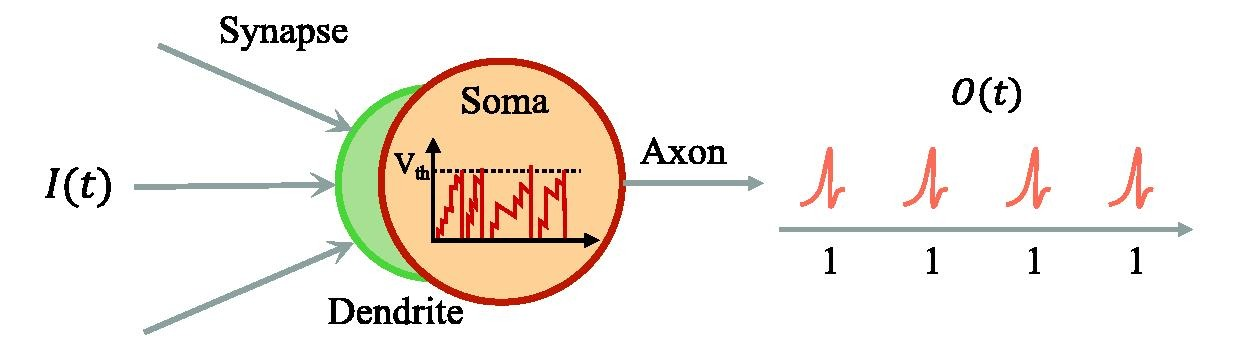
\includegraphics{image/neuronmodel.jpg}
        \caption{Neuron model basis\cite{LIAO2023126470}}
        \label{fig:neuronmodel}
      \end{center}
    \end{figure}
  \end{minipage}
  \hspace{0.5cm}
  \begin{minipage}{0.5\textwidth}
    \begin{center}
      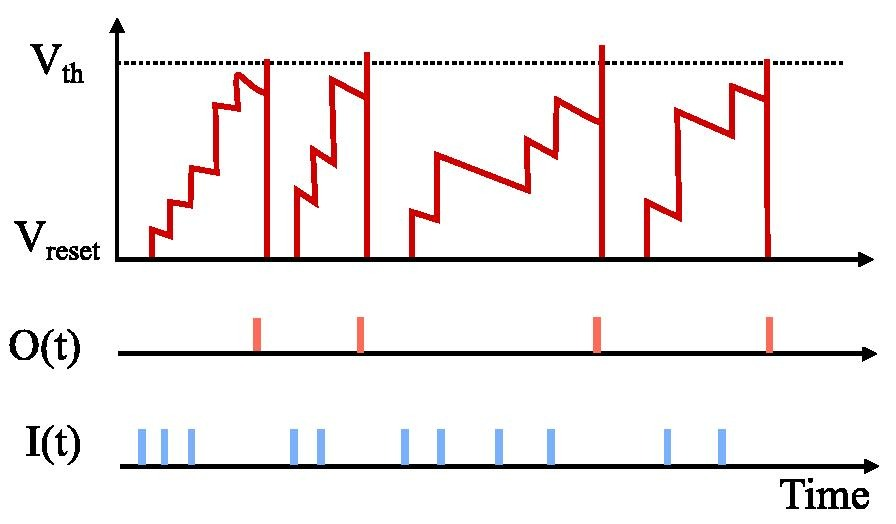
\includegraphics{image/generating_spikes.jpg}
      \caption{Generating spikes\cite{LIAO2023126470}}
      \label{fig:generating_spikes}
    \end{center}
  \end{minipage}
\end{figure}

% algo LIF
\subsubsection*{Small code example}
The algorithm defining the Lif neuron model in Snntorch have the following structure :
\begin{algorithm}[H]
  \caption{Snntorch : Leaky Integrate-and-Fire Neuron Model}
  \begin{algorithmic}[1]
    \Require $input$, $mem_0$
    \State Initialize $beta$, $threshold$, $spike\_grad$, $surrogate\_disable$, $init\_hidden$, $inhibition$, $learn\_beta$, $learn\_threshold$, $reset\_mechanism$, $state\_quant$, $output$
    \State Initialize $Leaky.beta$ and $Leaky.threshold$ if they are learnable
    \For{each $input$ in $batch$}
    \If{$reset\_mechanism = "subtract"$}
    \EndIf
    \State Compute $U[t+1] = \beta U[t] + I_{in}[t+1] - RU_{thr}$ if $reset\_mechanism = "subtract"$
    \State Compute $U[t+1] = \beta U[t] + I_{syn}[t+1] - R(\beta U[t] + I_{in}[t+1])$ if $reset\_mechanism = "zero"$
    \State Compute $spk$ and $mem_1$ for each element in the batch
    \State Return $spk$ and $mem_1$
    \EndFor
  \end{algorithmic}
\end{algorithm}

Here, the `reset\_mechanism` parameter is used to define the way the membrane potential is reset, for instead :
\begin{itemize}
  \item If `reset\_mechanism` is set to "subtract", the membrane potential will be reset to $0$ when the threshold is reached
  \item If `reset\_mechanism` is set to "zero", the membrane potential will be reset to $\beta U[t] + I_{in}[t+1]$ when the threshold is reached
\end{itemize}

In practice, when using Snntorch we would use 3 arrays to define this neuron model :

\begin{figure}[H]
  \begin{center}
    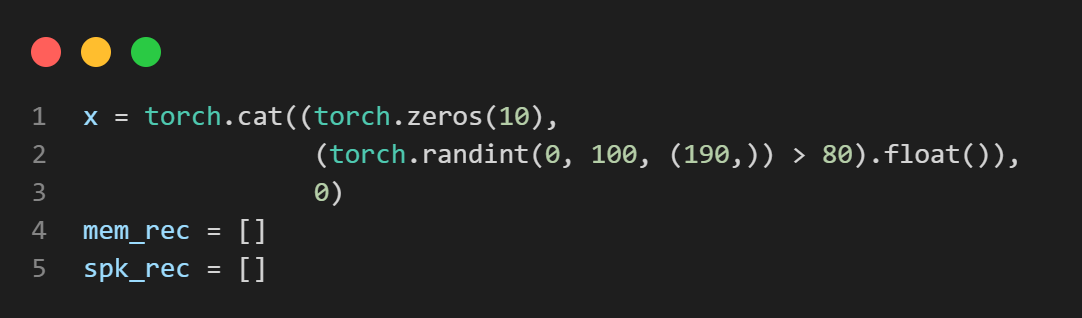
\includegraphics[width=\textwidth]{image/def_vars.png}
    \caption{Definition of the variables used in the LIF model}
    \label{fig:def_vars}
  \end{center}
\end{figure}

Where $x$ is the input, a tensor made (here) of $100$ elements, followed by an alternative of $0$ and $1$ (to mimic the spikes) randomly generated (here max of $80$). The membrane potential record $mem_{rec}$ is a list that will record the membrane potential at each time step and the spikes record $spk_{rec}$ is a list that will record the spikes at each time step.

Once the initialization is done (including some other parameters $\beta = \exp{- \frac{\Delta t}{\tau}} = 0.819$ and $W = 0.4 \in \mathbb{R}$), we can run the simulation for every time step.

\begin{figure}[H]
  \begin{center}
    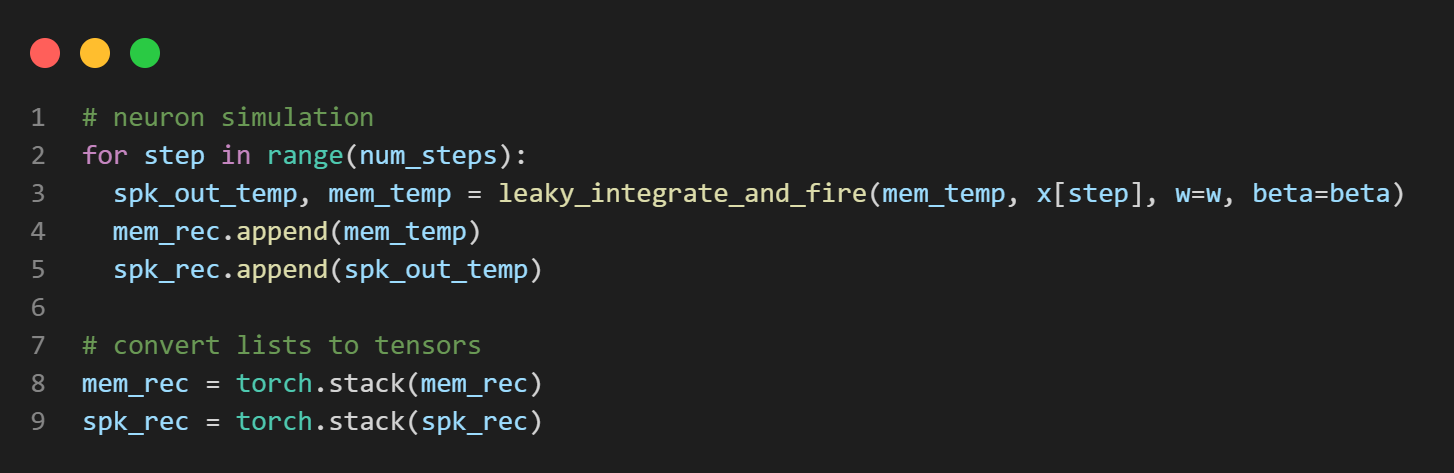
\includegraphics[width=\textwidth]{image/lif_example.png}
    \caption{Simulation of the LIF model}
    \label{fig:lif_sim}
  \end{center}
\end{figure}

And we get the following results :

\begin{itemize}
  \item At the top of the image the input $x$ is shown
  \item In the middle of the image the membrane potential $mem_{rec}$ is shown
  \item At the bottom of the image the spikes $spk_{rec}$ are shown
\end{itemize}

\begin{figure}[H]
  \begin{center}
    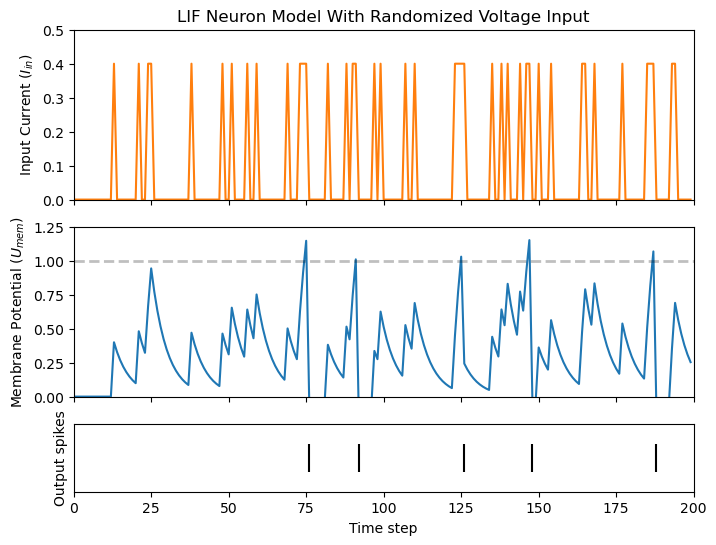
\includegraphics[width=0.8\textwidth]{image/output_lif1.png}
    \caption{Result of the simulation of the LIF model}
    \label{fig:lif_res}
  \end{center}
\end{figure}

\subsection{Spiking Neural Networks}



Now that the spiking neuron model is defined, we can create a network. The network is a mix between classic layers (for example fully connected layer) and spiking layers. Firstly a spiking layer needs to encode the data into spikes, which are then processed by the other layer. In some way, spiking layers will "take the place" of activation functions in CNN.





\hfill


\subsubsection{Loss}
To train the model, we use the cross entropy loss. With rate encoding the spike for the correct class is encouraged to produce a spike at each time step where the other are suppressed.

To compute the loss with $N_c$ classes, first the number of spikes is counted for each output neuron. With a spike count of output layer $\vec{c}$, we compute the softmax of spike count for each neuron.

$$ p_i = \frac{e^{c_i}}{\sum_{i=1}^{N_c} e^{c_i}} $$

The cross entropy between $p_i$ and the target $y_i \in \{0, 1\}$, which is a one-hot target vector, is obtained using:

$$ LCE = \sum_{i=0}^{N} y_i \log(p_i) $$



\begin{figure}[H]
  \centering
  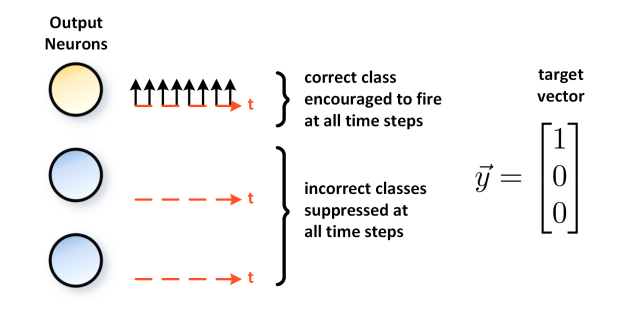
\includegraphics[width=\textwidth]{./image/loss_cross_entropy_snn_train.png}
  \caption{Output layer with rate coding, target vector is a one-hot encoded vector}
  \label{fig:snn_output}
\end{figure}


In the general scenario, the more spikes an output neuron is firing when compared to the others, the more likely it is to be the predicted class.


\subsection{Convolutional Spiking Neural Networks}

A convolutional Spiking neural network, or CSNN, is a particular case of SNN where the data pass into convolutional spiking layers to extract meaningful features.


\begin{figure}[H]
  \centering
  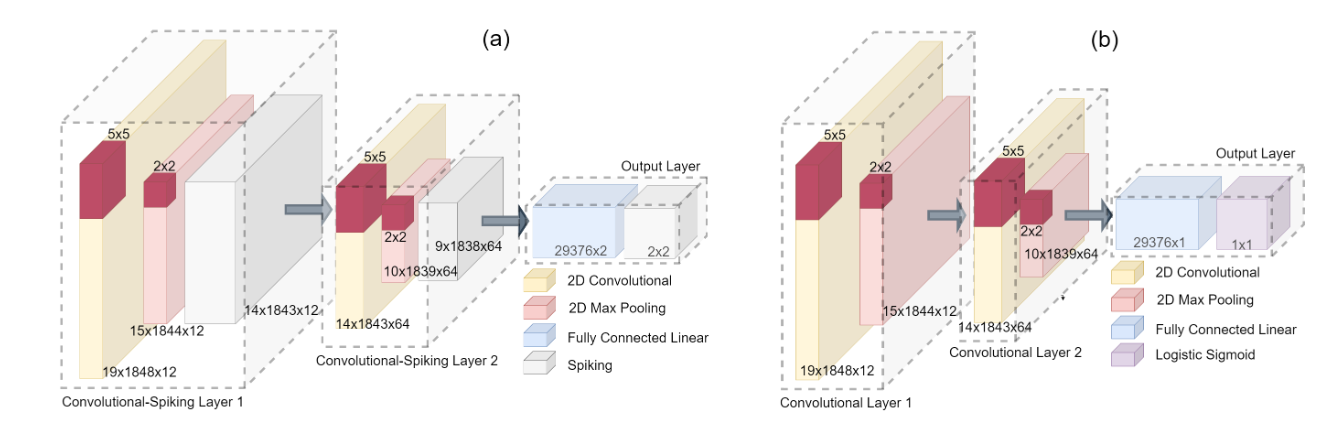
\includegraphics[width=\textwidth]{./image/csnn_template.png}
  \caption{(a) CSNN model, (b) CNN model}
  \label{fig:csnn_template}
\end{figure}

\pagebreak

\section{SNN - Behind the scenes}

\subsection{How to train a SNN}

\subsubsection{Dead Neuron Problem}

\begin{wrapfigure}{r}{0.6\textwidth}
  \centering
  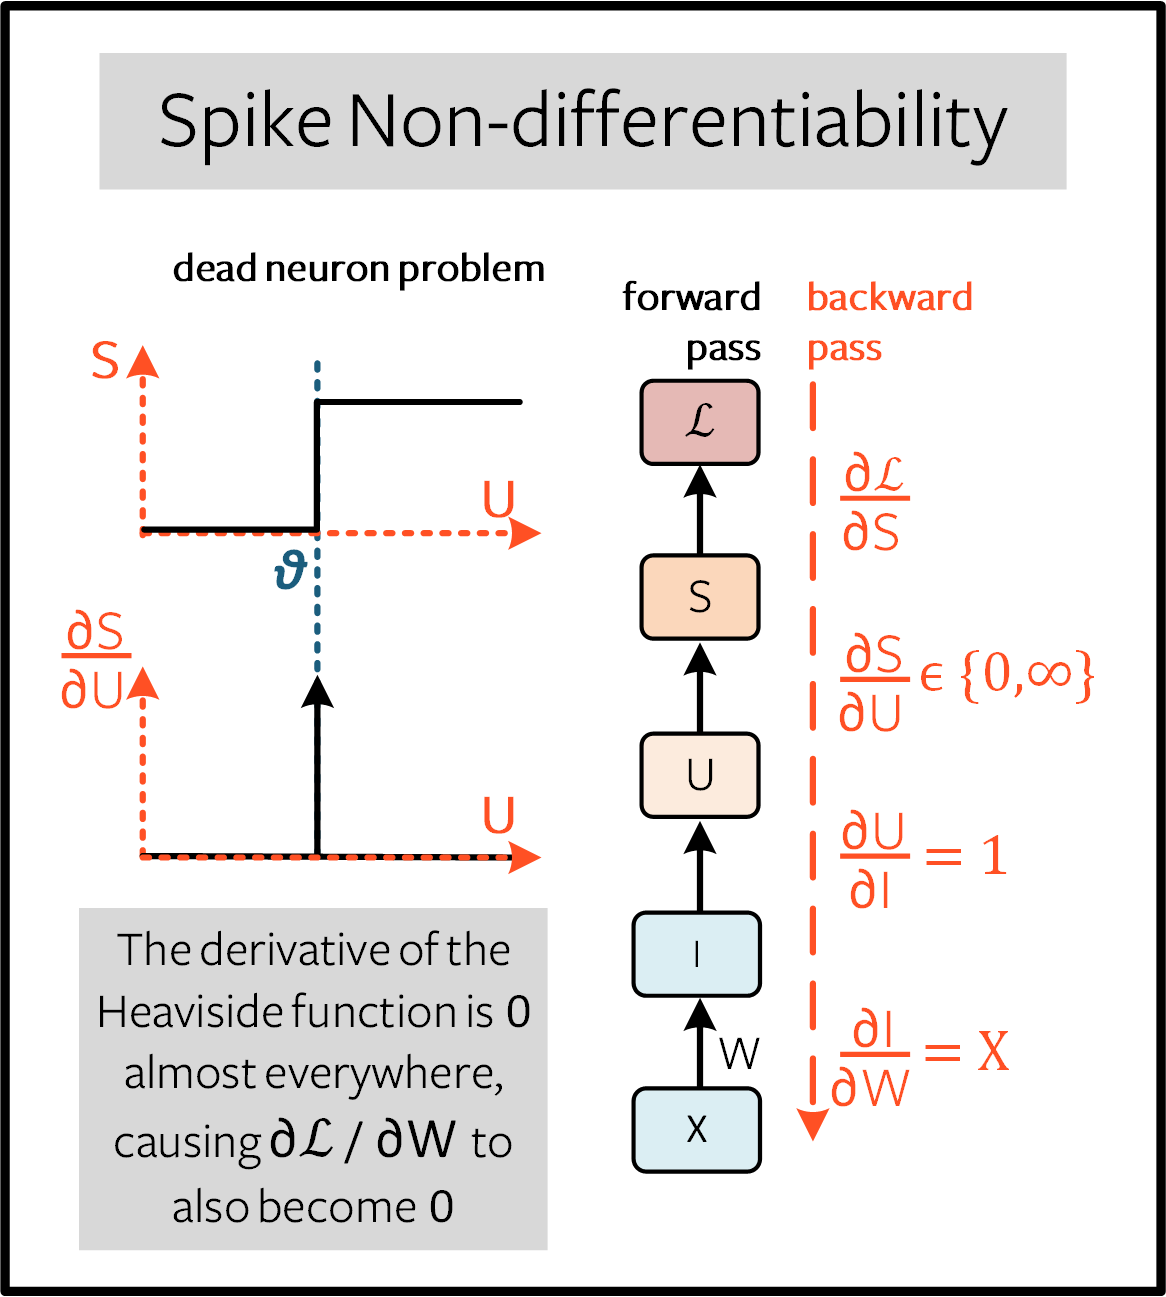
\includegraphics[width=0.6\textwidth]{./image/non-differentiability.png}
  \caption{Dead neuron problem\cite{eshraghian2021training}}
\end{wrapfigure}

To train a spiking neural network, we aim to adjust the weights based on the loss gradient, minimizing the overall loss. Backpropagation achieves this through a chain of derivatives (for one single time step):

\begin{equation}
  \frac{\partial \mathcal{L}}{\partial W} =
  \frac{\partial \mathcal{L}}{\partial S}
  \underbrace{\frac{\partial S}{\partial U}}_{\{0, \infty\}}
  \frac{\partial U}{\partial I}
  \frac{\partial I}{\partial W}
\end{equation}

Here, $\mathcal{L}$ is the loss, $W$ represents weights, $S$ is the output, $U$ is the activation function, and $I$ is the input.

The challenge lies in the term $\frac{\partial S}{\partial U}$, which takes values between $0$ and $\infty$. The derivative of the Heaviside step function from the input ($U$) is the Dirac Delta function. This function is $0$ everywhere except at the threshold $\theta$, where it tends to infinity. Consequently, the gradient is often nullified to zero (or saturated if $\theta$ precisely aligns with the threshold), hindering learning. This issue is commonly known as the \textbf{dead neuron problem}. There are multiple ways to address this issue.

\subsection{Shadow training}

In shadow training, a classic ANN is trained and converted into an SNN by interpreting the "excitation" of the activation function as a firing rate (rate coding) or spike time (latency coding). The goal is to achieve the same input-output mapping with a deep SNN as the original ANN. This is very practical because it doesn't need particular knowledge about SNNs for the training. However, it has some flaws, for example one major obstacle is that in ANNs it does not matter if activations are negative, whereas firing rates in SNNs are always positive.\cite{pfeiffer2018}

\subsection{Surrogate Gradient}

One way to address this non-differentiability issue would be to compute a gradient on a "relaxed" version of the non-differentiable function. This would mean approximating the Heaviside step function $S(U)$ with a differentiable function $f(U)$, such as the sigmoid function or the $\arctan$ function. For example:

\begin{figure}[H]
  \begin{minipage}[t]{0.5\textwidth}
    \vspace{40pt} % Adjust this value as needed
    $$\begin{aligned}
        %Heaviside step function
        S(U)   & = \begin{cases}
                     0 & \text{if } U < U_{\rm thr}    \\
                     1 & \text{if } U \geq U_{\rm thr}
                   \end{cases}                                                                  \\ \\
        S(U)   & \approx \frac{1}{1 + e^{-(U - U_{\rm thr})}}                                                         \\
        S(U)   & \approx \frac{1}{\pi} \arctan((U - U_{\rm thr})) + \frac{1}{2}                                       \\
        % Fast sigmoid
        S_k(U) & \approx \frac{1}{2} \frac{U - U_{\rm thr}}{\sqrt{1 + k \lvert U - U_{\rm thr} \rvert}} + \frac{1}{2}
      \end{aligned}$$
  \end{minipage}
  \hfill
  \begin{minipage}[t]{0.45\textwidth}
    \vspace{0pt} % Adjust this value as needed
    \centering
    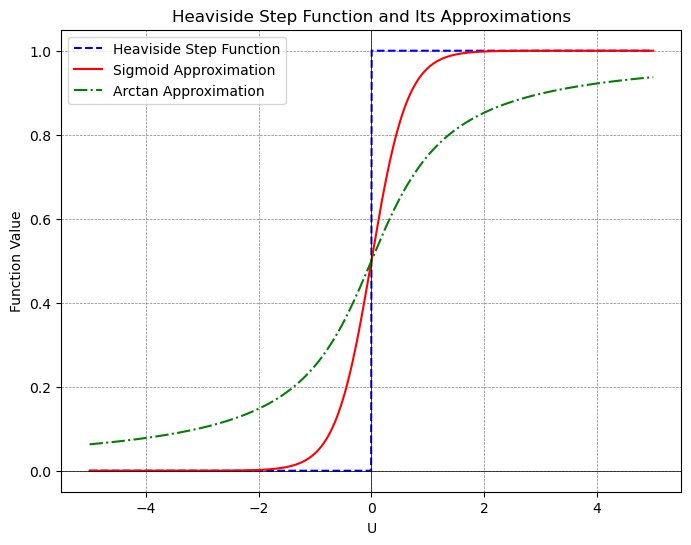
\includegraphics[width=\textwidth]{./image/approx_surrogate.png}
    \caption{Visualization of the Heaviside step function approximation\cite{LIAO2023126470}}
    \label{fig:approx_surrogate}
  \end{minipage}
\end{figure}

This solution should only account for the backpropagration process. Indeed, we only need to approximate the derivative of the Heaviside step function, not the function itself. The approximation of the function is only used to compute the gradient, and the original function is used to compute the output of the neuron.

\subsubsection{Loss function treatment}

In order for this to be taken into account in the loss function (and because we now have to take the time as a parameter), we have to perform an operation on the loss function for all its time steps.

\begin{equation}
  \frac{\partial \mathcal{L}}{\partial W}=\sum_t \frac{\partial\mathcal{L}[t]}{\partial W} =
  \sum_t \sum_{s\leq t} \frac{\partial\mathcal{L}[t]}{\partial W[s]}\frac{\partial W[s]}{\partial W}
\end{equation}

In the above equation, we ensure causality by summing over all time steps $t$ and all previous time steps $s$. We thereby make the assumption that the weights at time $s \in \left[\|0, t \|\right]$ influence the weights at time $t$.

\begin{itemize}
  \item We define as \textit{prior influence} the influence of the weights at time $s < t$ on the weights at time $t$.
  \item We define as \textit{immediate influence} the influence of the weights at time $t$ on the weights at time $t$.
\end{itemize}

A recurrent system constrains the weight to be shared across all steps: $W[0]=W[1] =~... ~ = W$. Therefore, a change in $W[s]$ will have the same effect on all $W$, which implies that
$\partial W[s]/\partial W=1$:

\begin{equation}
  \frac{\partial \mathcal{L}}{\partial W}=
  \sum_t \sum_{s\leq t} \frac{\partial\mathcal{L}[t]}{\partial W[s]}
\end{equation}

By performing a chain rule, we can express the derivative of the loss with respect to the weights at time $s$ as:

\begin{figure}[H]
  \begin{minipage}{0.5\textwidth}
    \centering
    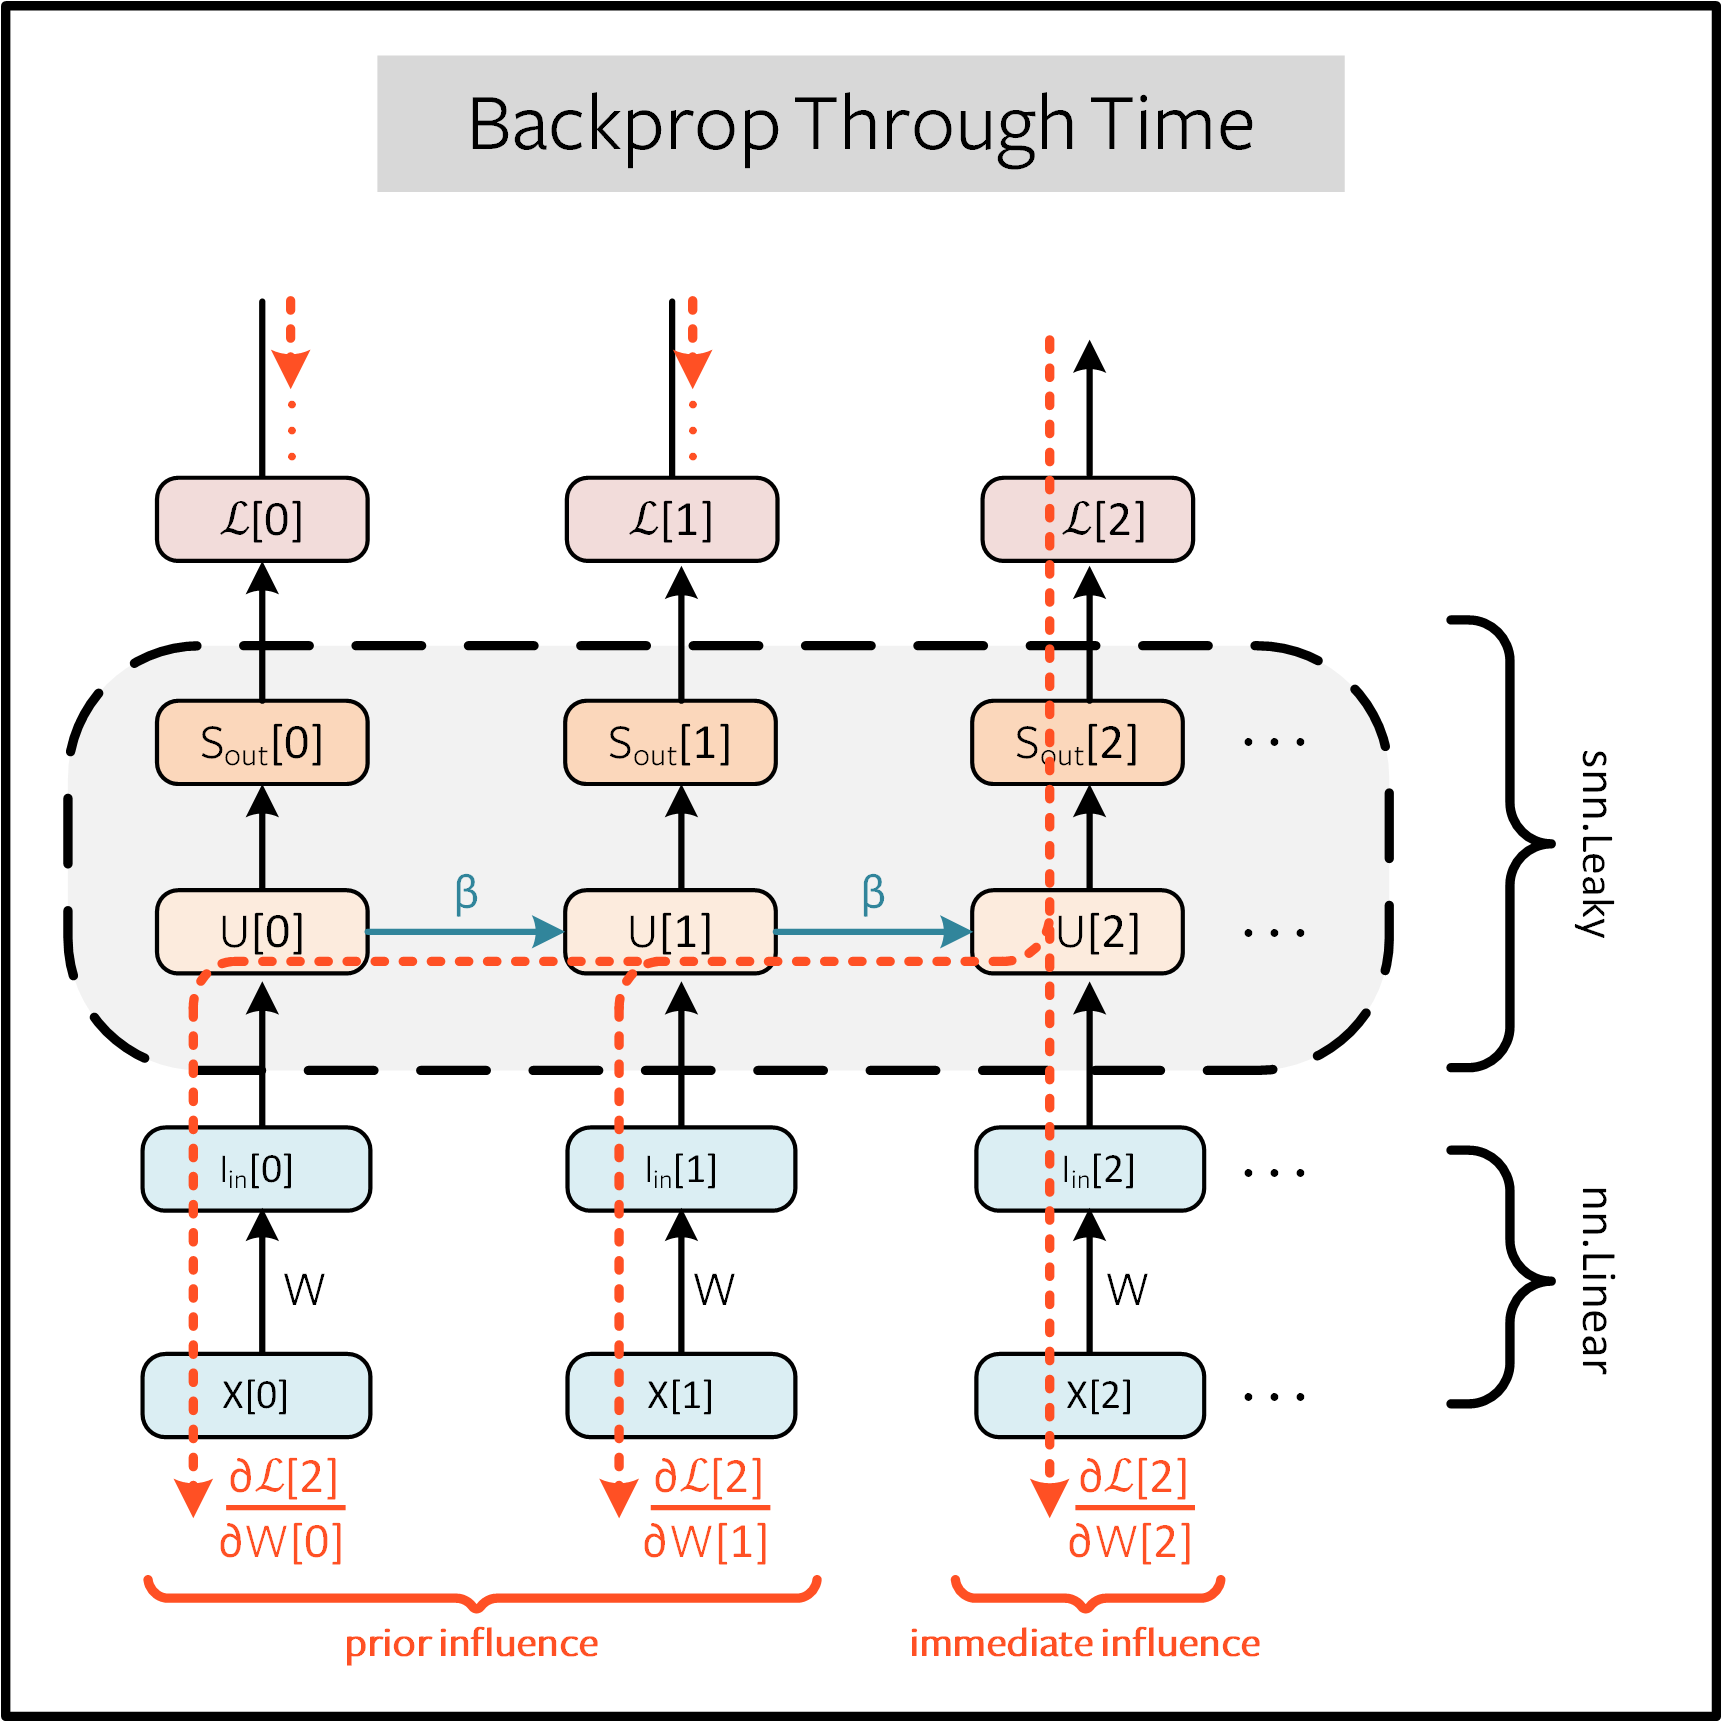
\includegraphics[width=\textwidth]{image/bptt.png}
    \caption{Backpropagation through time}
    \label{fig:bptt}
  \end{minipage}
  \hspace{0.5cm}
  \begin{minipage}{0.5\textwidth}
    \begin{equation*}
      \begin{aligned}
        \frac{\partial \mathcal{L}[t]}{\partial W[t-1]} & =
        \frac{\partial \mathcal{L}[t]}{\partial S[t]}
        \underbrace{\frac{\partial \tilde{S}[t]}{\partial U[t]}}_{Eq.~(5)}
        \underbrace{\frac{\partial U[t]}{\partial U[t-1]}}_\beta
        \underbrace{\frac{\partial U[t-1]}{\partial I[t-1]}}_1
        \underbrace{\frac{\partial I[t-1]}{\partial W[t-1]}}_{X[t-1]} \\
        \frac{\partial \mathcal{L}[t]}{\partial W[t-2]} & =
        \frac{\partial \mathcal{L}[t]}{\partial S[t]}
        \underbrace{\frac{\partial \tilde{S}[t]}{\partial U[t]}}_{Eq.~(5)}
        \underbrace{\frac{\partial U[t]}{\partial U[t-2]}}_{\beta^2}
        \underbrace{\frac{\partial U[t-2]}{\partial I[t-2]}}_1
        \underbrace{\frac{\partial I[t-2]}{\partial W[t-2]}}_{X[t-2]} \\
                                                        & \vdots      \\
        \frac{\partial \mathcal{L}[t]}{\partial W[0]}   & =
        \frac{\partial \mathcal{L}[t]}{\partial S[t]}
        \underbrace{\frac{\partial \tilde{S}[t]}{\partial U[t]}}_{Eq.~(5)}
        \underbrace{\frac{\partial U[t]}{\partial U[0]}}_{\beta^t}
        \underbrace{\frac{\partial U[0]}{\partial I[0]}}_1
        \underbrace{\frac{\partial I[0]}{\partial W[0]}}_{X[0]}
      \end{aligned}
    \end{equation*}
  \end{minipage}
\end{figure}
\pagebreak

\section{Practical implementation}

Let us now present a small program showcasing our results.
In this section, we aim to show some of the results we had and their meaning in the context of the project.

\subsection{Defining studied models}

We defined 2 SNN models during the last full time period of the project. The first one is a simple feedforward SNN, and the second one is a convolutional SNN. We also defined the same models but with the ANN architecture, and also tried some other kownn architectures for comparison. Respectively:

\subsubsection{SNN}

\subsubsection*{Simple SNN for looking at spikes}

A feedforward SNN with the following struture :
\begin{figure}[H]
  \begin{minipage}{0.4\textwidth}
    \centering
    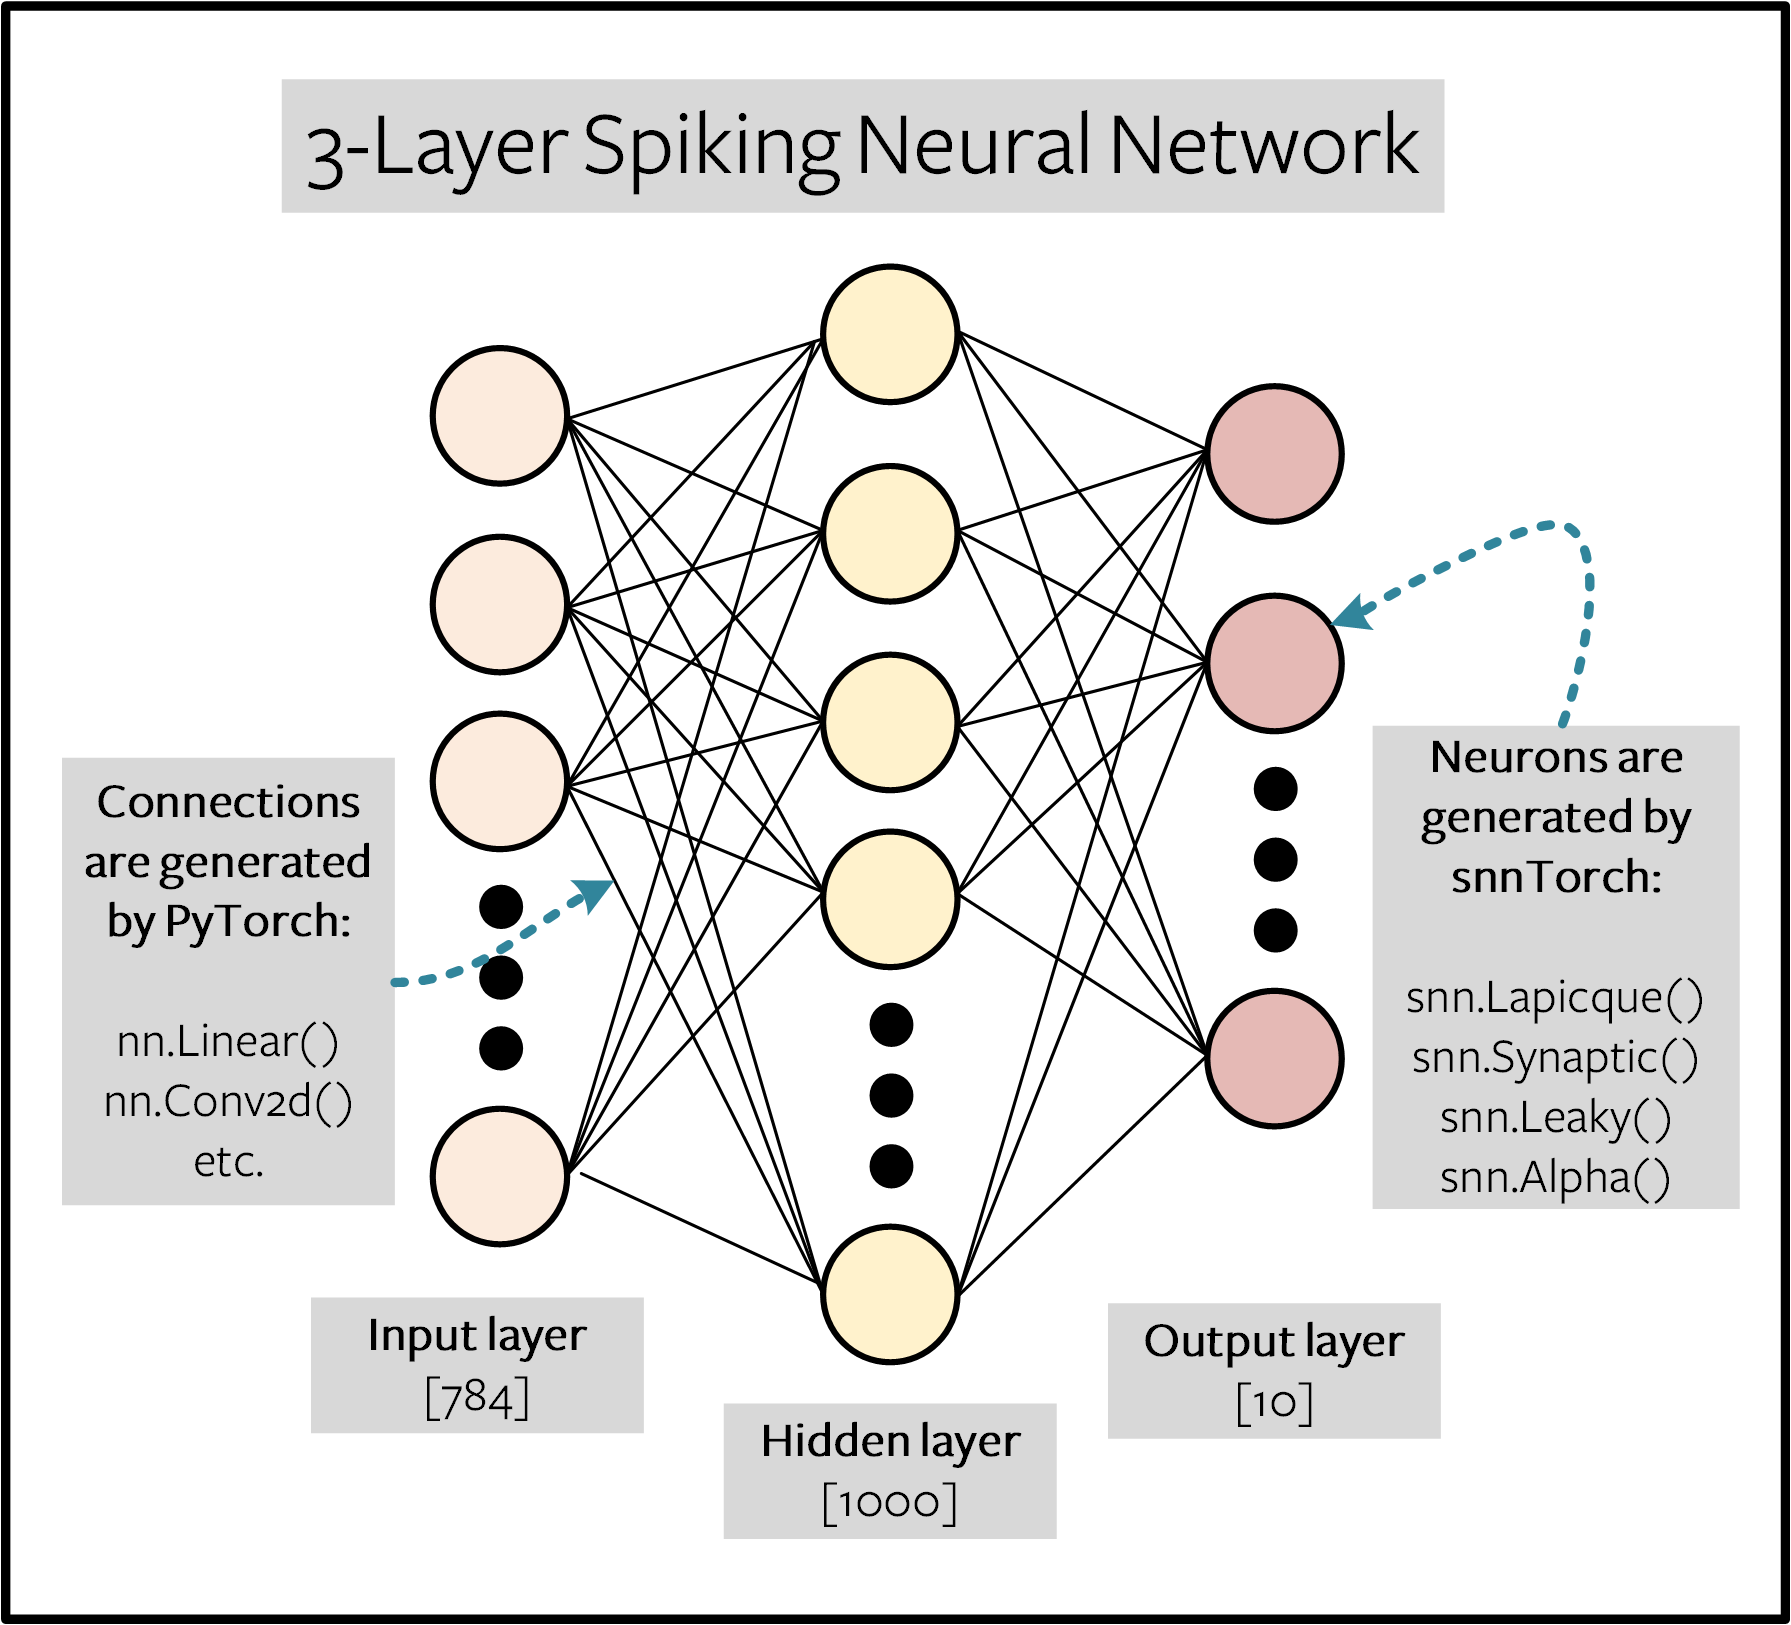
\includegraphics[width=0.9\linewidth]{image/2_8_fcn.png}
    \caption{Simple SNN}
    \label{fig:simple_snn}
  \end{minipage}
  \begin{minipage}{0.5\textwidth}
    \centering
    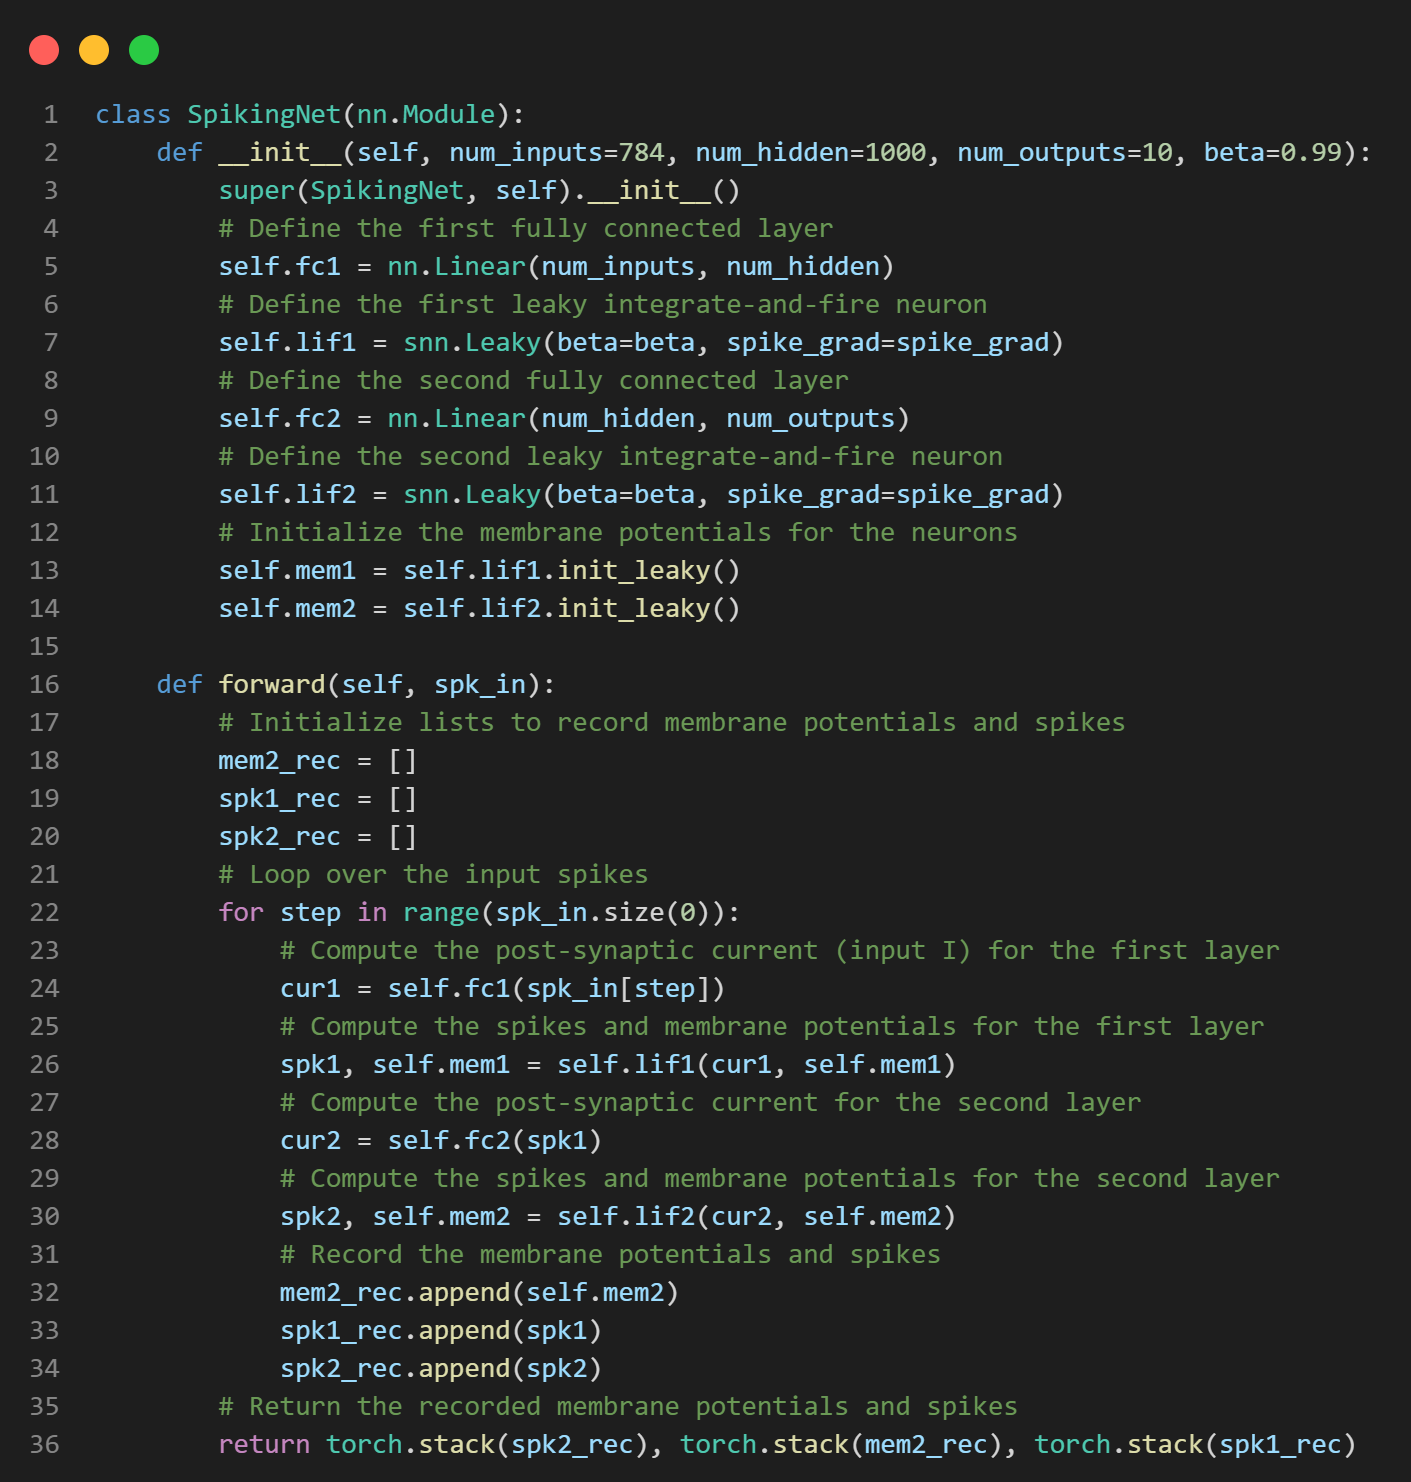
\includegraphics[width=\linewidth]{image/2_8_fcn_code.png}
    \caption{Simple SNN}
    \label{fig:simple_snn_code}
  \end{minipage}
\end{figure}

\subsubsection*{CSNN}

\hyperref[fig:csnn_template]{The above} convolutionnal spiking neural network :

\begin{figure}[H]
  \begin{minipage}{0.4\textwidth}
    \centering
    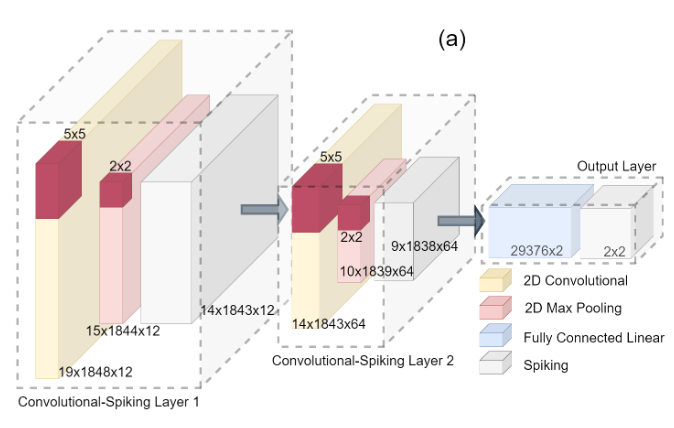
\includegraphics[width=0.9\linewidth]{image/csnn_template_model.png}
  \end{minipage}
  \begin{minipage}{0.6\textwidth}
    \centering
    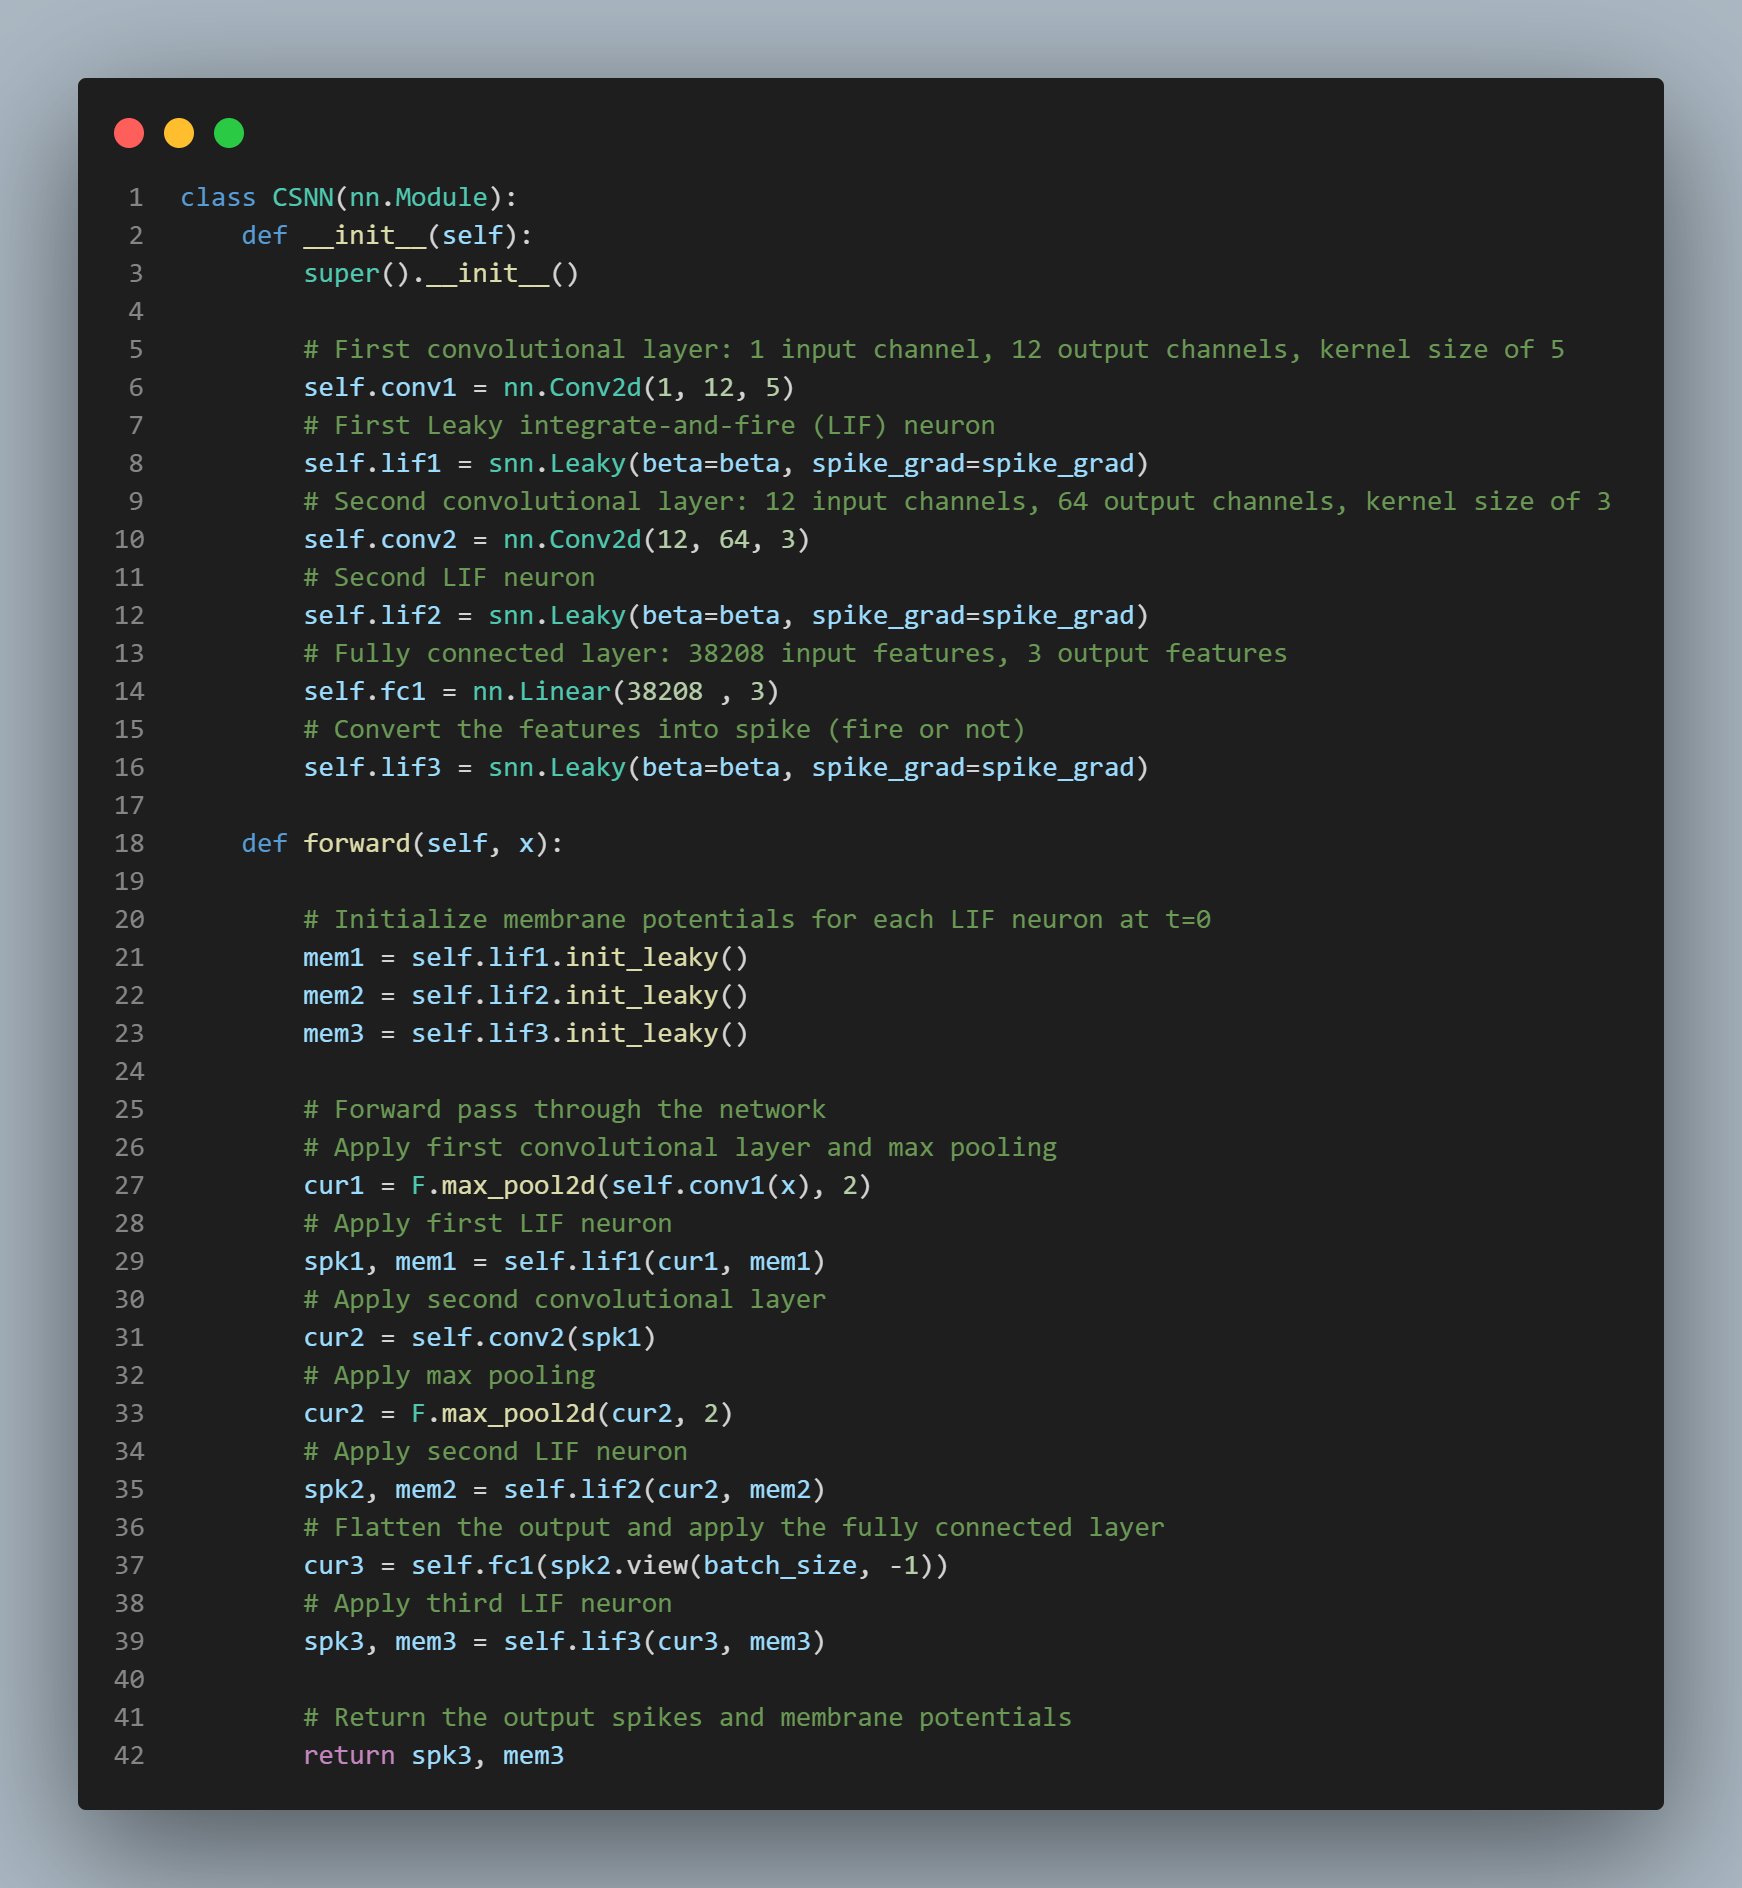
\includegraphics[width=\textwidth]{./image/csnn_code.png}    \caption{CSNN code}
    \label{fig:csnn_code}

  \end{minipage}
\end{figure}

\subsubsection{ANNs}

To make some comparison, we also defined the same models but with the ANN architecture, and also tried some other kownn architectures for comparison. Respectively:

\begin{itemize}
  \item The equivalent ANN for our CSNN model.
  \item RESNET50, RESNET101
  \item EFFICIENTNET-B0
  \item VGG16
  \item Densenet 121
  \item MobileNetV2
\end{itemize}

Please note that some parameters like the number of MFCC features may vary between the ANNs and the CSNN usage, due to memory usage issues.

\pagebreak

\subsection{Results on MNIST}

When we worked with the MNIST dataset, we only worked with spiking neural networks.

\subsubsection*{Feedforward SNN}

Firstly we issued some illustrations on what proportion of the input data (converted into spiking data) was transmitted, layer by layer. This gave us the bellow results, the fist line corresponds to the rate encoding of the input data, the second line corresponds to the spikes emitted by the first layer, and the last spike corresponds to the spikes emitted by the output layer (all stacked in an image).
\begin{figure}[H]
  \begin{minipage}{0.5\textwidth}
    \begin{center}
      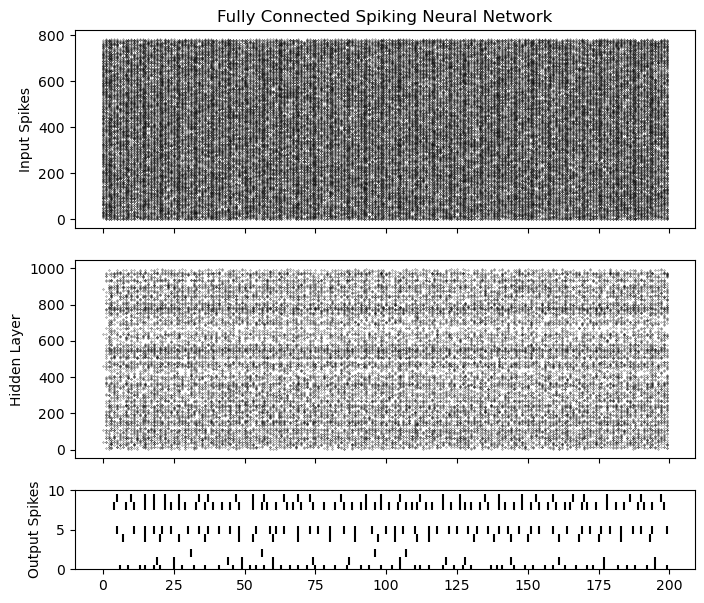
\includegraphics[width=0.75\textwidth]{image/spikes_simple_snn.png}
      \caption{Observation of spikes after rate encoding and after each LiF layers}
      \label{fig:spikes_snn}
    \end{center}
  \end{minipage}
  \hspace{0.5cm}
  \begin{minipage}{0.5\textwidth}
    \begin{center}
      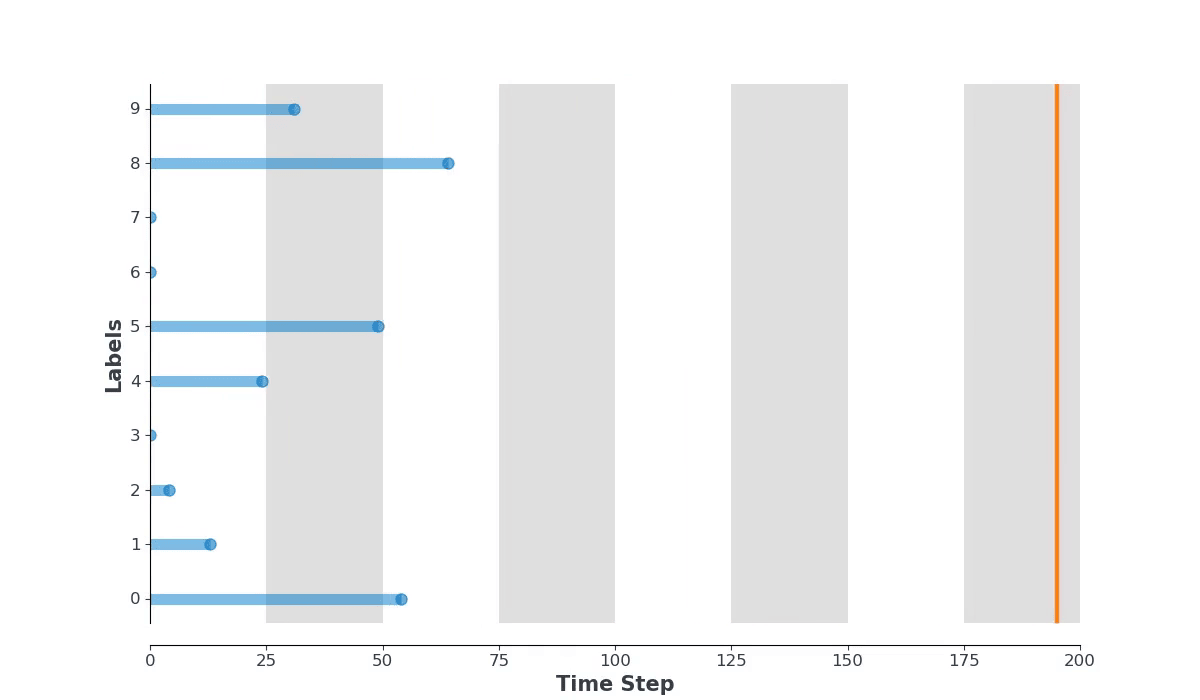
\includegraphics[width=\textwidth]{image/mnist1_050.png}
      \caption{Last image of a prediction of the SNN model on the MNIST dataset (not trained)}
      \label{fig:mnist1}
    \end{center}
  \end{minipage}
\end{figure}

From top to bottom of \hyperref[fig:mnist1]{figure 24}, we observe the clear reduction of the number of spikes emitted. Also note that this model was not trained and was only used to observe the spikes.

\subsubsection*{Convolutional SNN}

When training the CSNN model (having far less parameters than the previous one), we obtained the following results:

\begin{figure}[H]
  \begin{minipage}{0.5\textwidth}
    \begin{center}
      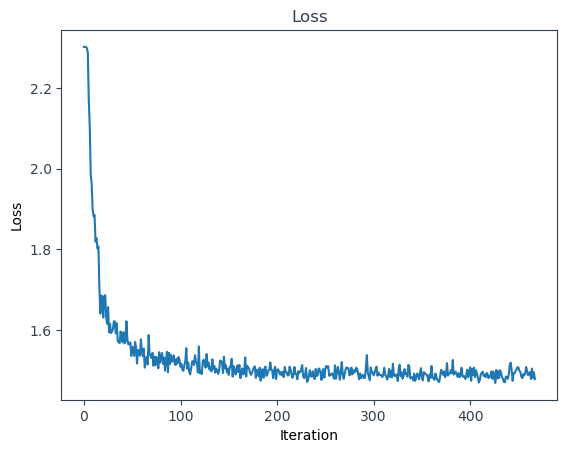
\includegraphics[width=\textwidth]{image/loss_MNIST.png}
      \caption{Loss of the CSNN model on the MNIST dataset}
      \label{fig:loss_MNIST}
    \end{center}
  \end{minipage}
  \hspace{0.5cm}
  \begin{minipage}{0.5\textwidth}
    \begin{center}
      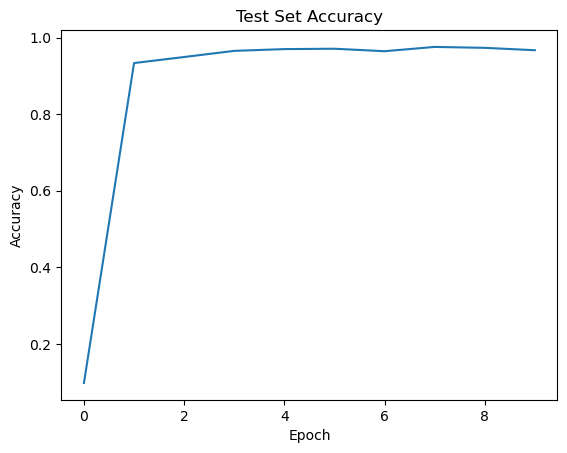
\includegraphics[width=\textwidth]{image/accuracy_MNIST.png}
      \caption{Accuracy of the CSNN model on the MNIST dataset}
      \label{fig:accuracy_MNIST}
    \end{center}
  \end{minipage}
\end{figure}

\begin{figure}[H]
  \begin{center}
    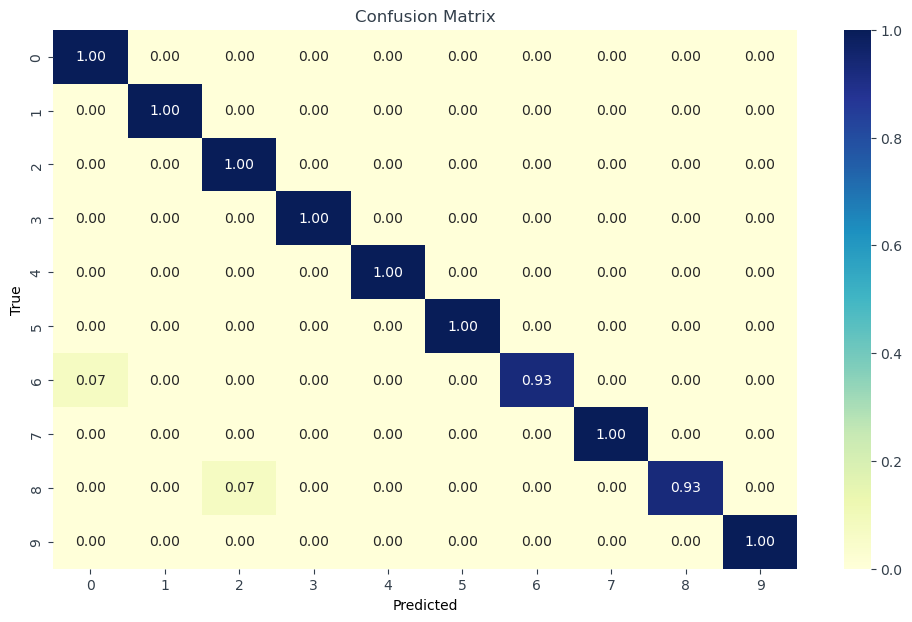
\includegraphics[width=\textwidth]{image/confusion_mat_MNIST.png}
    \caption{Confusion matrix of the CSNN model on the MNIST dataset}
    \label{fig:confusion_matrix_MNIST}
  \end{center}
\end{figure}


\begin{figure}[H]
  \begin{center}
    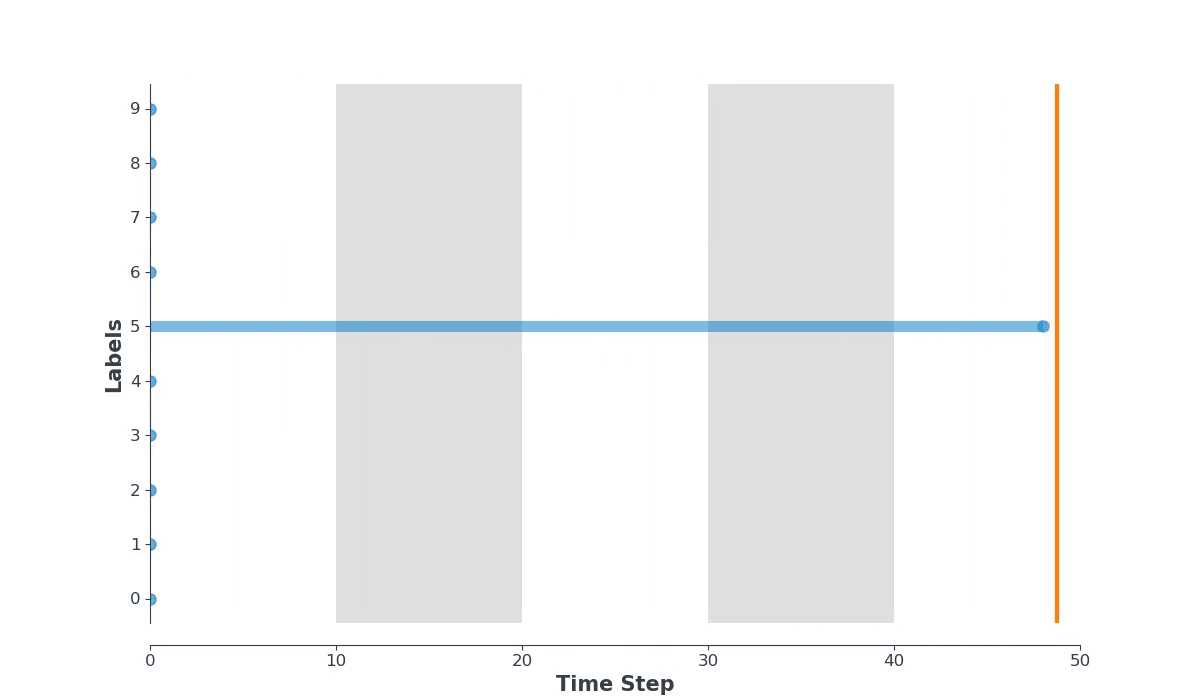
\includegraphics[width=\textwidth]{image/mnist2_050.png}
    \caption{Last image of a prediction of the CSNN model on the MNIST dataset}
    \label{fig:mnist2}
  \end{center}
\end{figure}

In this last image, we observe that the only neuron that fired for all time steps is the one associated to the predicted class $5$. We aim now to test the model on our test dataset and as similar results as possible (in term of efficiency).

\subsection{Our Dataset}

We used the Google AudioSet dataset as the basis for our audio classification task. The dataset is divided into 10-second audio clips, each labeled with one or multiple classes. The classes are organized in a hierarchical structure, with the top-level classes being broad categories like "Music" or "Speech", and the lower-level classes being more specific, like "Piano" or "Saxophone".

It is composed of csv files, each one containing some time codes and a link to a youtube video. In order to create an exploitable dataset out of this one, we used the following steps:

\begin{itemize}
  \item Divide the dataset into 3 csv files, each one associated to a top-level class (Music, Animals and Sound of things)
  \item Make sure there are no repetitions in between those classes
  \item Filter the dataset so that we keep "recognizable" sounds
  \item Perform some post-processing to make the dataset exploitable (outdated links, duration smaller than 10 seconds, etc.)
\end{itemize}

So we end up with 3 class files, each one containing a list of youtube links and their associated class (with most of the time other "noise" classes that are not to be taken into account for the classification task on high level classes). We then used the youtube-dl library to download the videos (parallel operations) and the soc library to extract the audio from the videos with the correct duration and format.

We decided to use this dataset to perform some audio classification because, we though that, as the dataset is quite large and, as it is a hierarchical dataset and its categories are quite diverse, it would be a good dataset to test the capabilities of spiking convolutional neural networks.
Furthermore, if the model we create performs well on this dataset, which is quite unbalanced and diverse, it would be a good sign that it could perform well on embedded systems, where the data has often this kind of characteristics.


\subsubsection{Mel-frequency cepstral coefficients (MFCC)}

After having imported the dataset, we needed to make it usable by the networks. We chose to convert it to MFCCs.

This approach is used in audio analysis to capture information specific to human auditory characteristics while reducing data redundancy. MFCCs thus encapsulate frequency variations over time in a compact way, producing a set of cepstral coefficients that are widely used for automatic speech recognition and other audio signal processing tasks.

Two of the main advantages of MFCCs are compactness and information discrimination. MFCCs condense information while preserving the signal's distinctive characteristics. Compact representation facilitates storage, transmission, and processing of large amounts of data.
By focusing on perceptual features rather than raw frequency, MFCCs are less sensitive to pitch variations, improving the robustness of sound recognition.

Some python libraries like librosa have functions to convert directly audio in MFCC. These are the steps to convert an audio signal in MFCC:

\begin{itemize}
  \item Take the signal's Short Term Fourier Transform (STFT), which divides the audio signal into multiple parts and compute the Fourier Transform for each one. In practice, we use the Discrete Fourier Transform.

        \begin{equation}
          STFT: \;\left\{ x[ n ] \right\} \equiv X(m,\omega) = \sum_{n=-\infty}^{\infty} x[n]w[n-m]\mathrm{e}^{-j \omega n}
        \end{equation}

  \item Map the powers of the resulting spectrum to the Mel scale, multiplying by overlapping window functions (triangular or cosine), then take the logarithm of the amplitudes at each mel frequency. The Mel scale is semi-logarithmic, to better represent actual human perception of frequencies.

        \begin{equation}
          Mel \; scale: \; m = 2595 \log_{10}\left(1 + \frac{f}{700}\right)
        \end{equation}

  \item Take the discrete cosine transform (DCT) of the list of logarithmic powers of the mel frequencies, as if it were a signal. The MFCCs are the amplitudes of the resulting spectrum.

        \begin{equation}
          DCT: \; S_{u,v} = \sum_{m = 0}^{M- 1} \sum_{n = 0}^{N- 1} s(m, n)\mathrm e^{-2\mathrm i\pi \left ( \frac{um}M+ \frac{vn}N\right )}
        \end{equation}

\end{itemize}



\subsection{Results and discussion}

\subsubsection*{ANNs}

\begin{figure}[H]
  \centering
  \subfloat[Loss CNN]{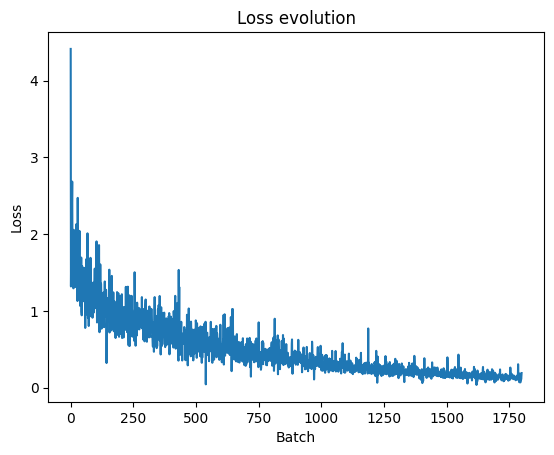
\includegraphics[width=0.3\textwidth]{image/loss_cnn.png}
    \label{fig:loss_cnn}}
  \hfill
  \subfloat[Accuracy CNN]{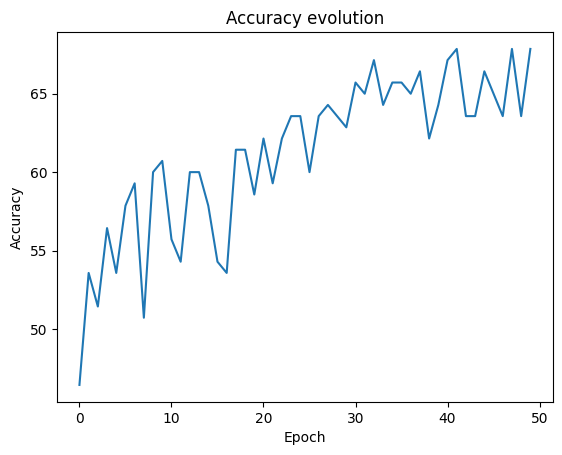
\includegraphics[width=0.3\textwidth]{image/acc_cnn.png}}
  \label{fig:acc_cnn}
  \hfill
  \subfloat[Confusion matrix CNN]{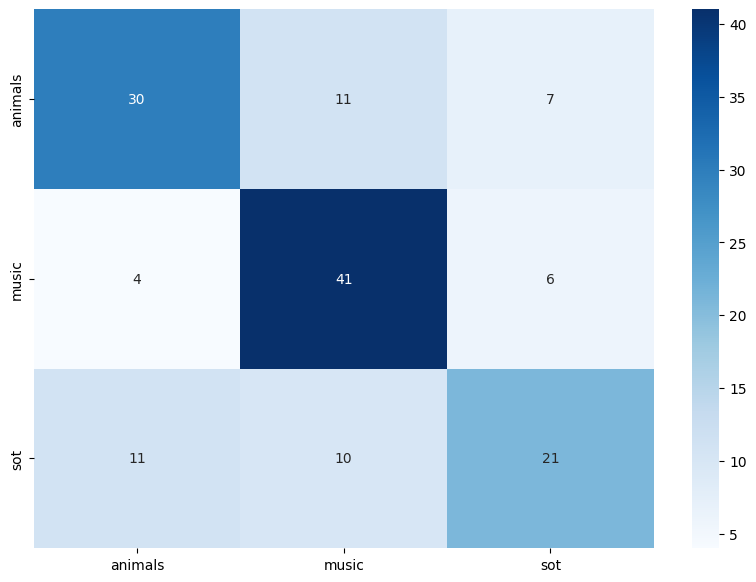
\includegraphics[width=0.3\textwidth]{image/conf_mat_cnn.png}
    \label{fig:conf_mat_cnn}}
  \\
  \subfloat[Loss RESNET50]{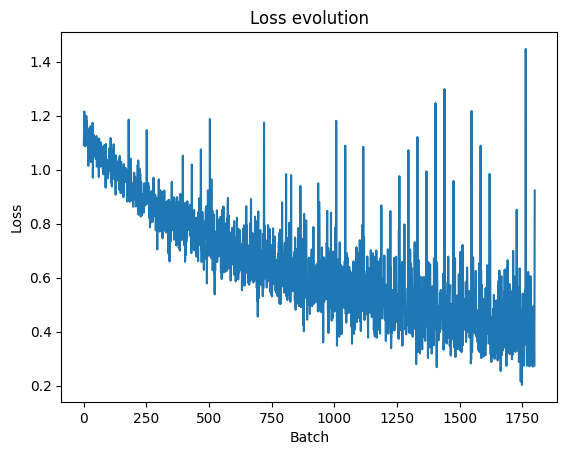
\includegraphics[width=0.3\textwidth]{image/loss_resnet.png}
    \label{fig:loss_resnet}}
  \hfill
  \subfloat[Accuracy RESNET50]{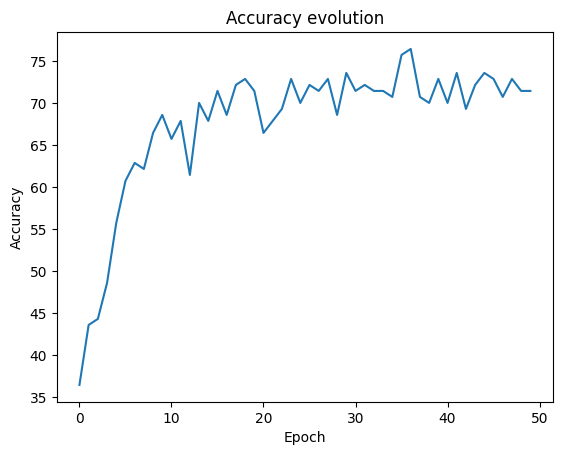
\includegraphics[width=0.3\textwidth]{image/acc_resnet.png}
    \label{fig:acc_resnet}}
  \hfill
  \subfloat[Confusion matrix RESNET50]{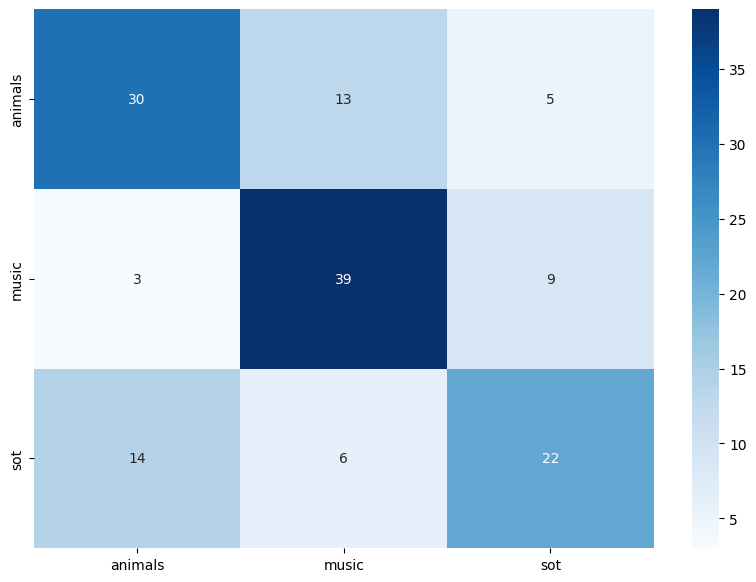
\includegraphics[width=0.3\textwidth]{image/conf_mat_resnet.png}
    \label{fig:conf_mat_resnet}}
  \\
  \subfloat[loss MobileNetV2]{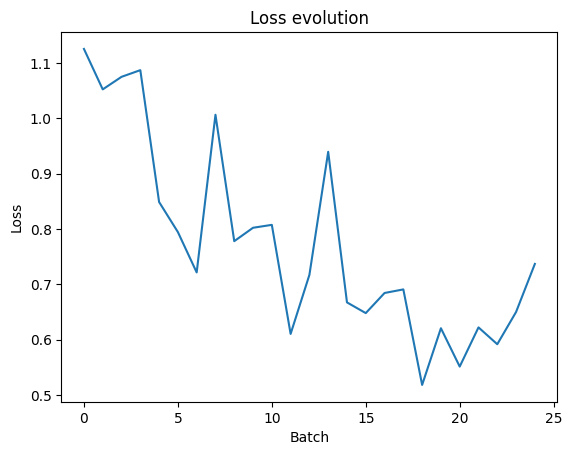
\includegraphics[width=0.3\textwidth]{image/loss_mobileV2.png}
    \label{fig:loss_mobileV2}}
  \hfill
  \subfloat[Accuracy MobileNetV2]{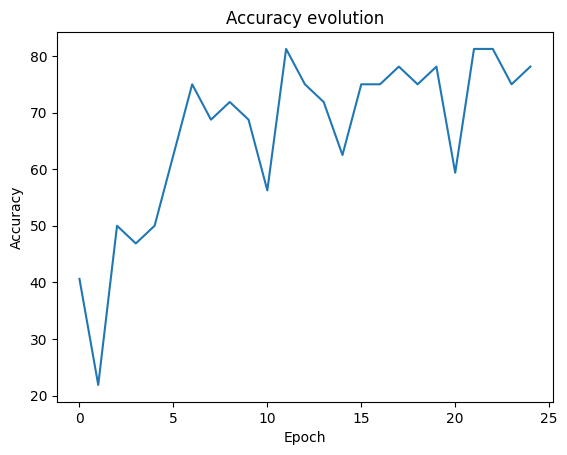
\includegraphics[width=0.3\textwidth]{image/acc_mobileV2.png}}
  \hfill
  \subfloat[Confusion matrix MobileNetV2]{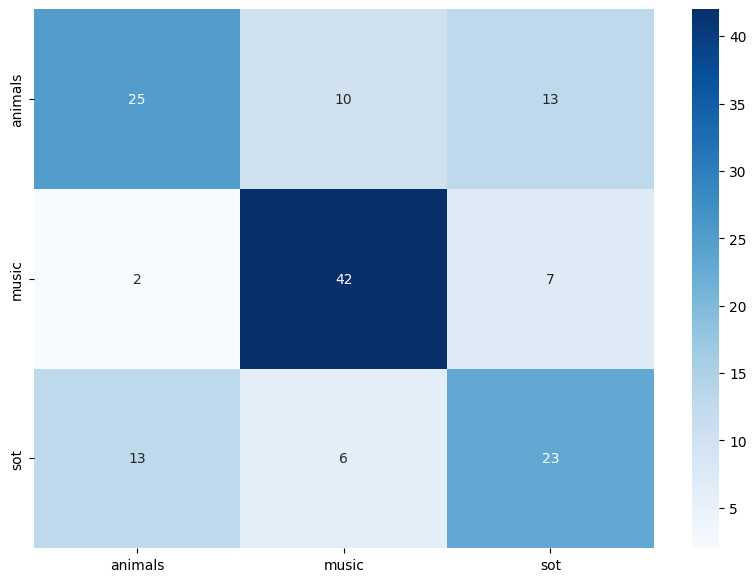
\includegraphics[width=0.3\textwidth]{image/conf_mat_mobileV2.png}}
  \label{fig:conf_mat_mobileV2}
  \caption{Results of the ANNs on the dataset (no data augmentation)}
  \label{fig:results_anns}
\end{figure}


\subsubsection*{SNNs}

We tried multiple way on training our CSNN model onto the dataset we made,



\pagebreak

% Bibliography
\bibliographystyle{siam}
\bibliography{ref}


\end{document}
